\documentclass[12pt, times new roman]{article}
\usepackage[utf8]{inputenc}
\usepackage{graphicx}

\title{Mahasiswa App}
\author{Heriyanto}
\date{October 2019}

\begin{document}

\maketitle
\section{Membuat aplikasi melalui apex.oracle}
Membuat aplikasi melalui apex oracle begitu mudah dan cepat, dengan salah satu fiturnya yaitu membuat aplikasi dengan file yang berbentuk atau berekstensi csv, xlsx, xml atau json yang sudah ada di komputer kita, dapat kita buat menjadi aplikasi di apex oracle.
\section{Langkah - Langkah Membuat Aplikasi di Apex Oracle}
\begin{itemize}
\item Pertama kita sediakan file excel yang sudah ada.
\begin{figure}[htbp]
	\centering
	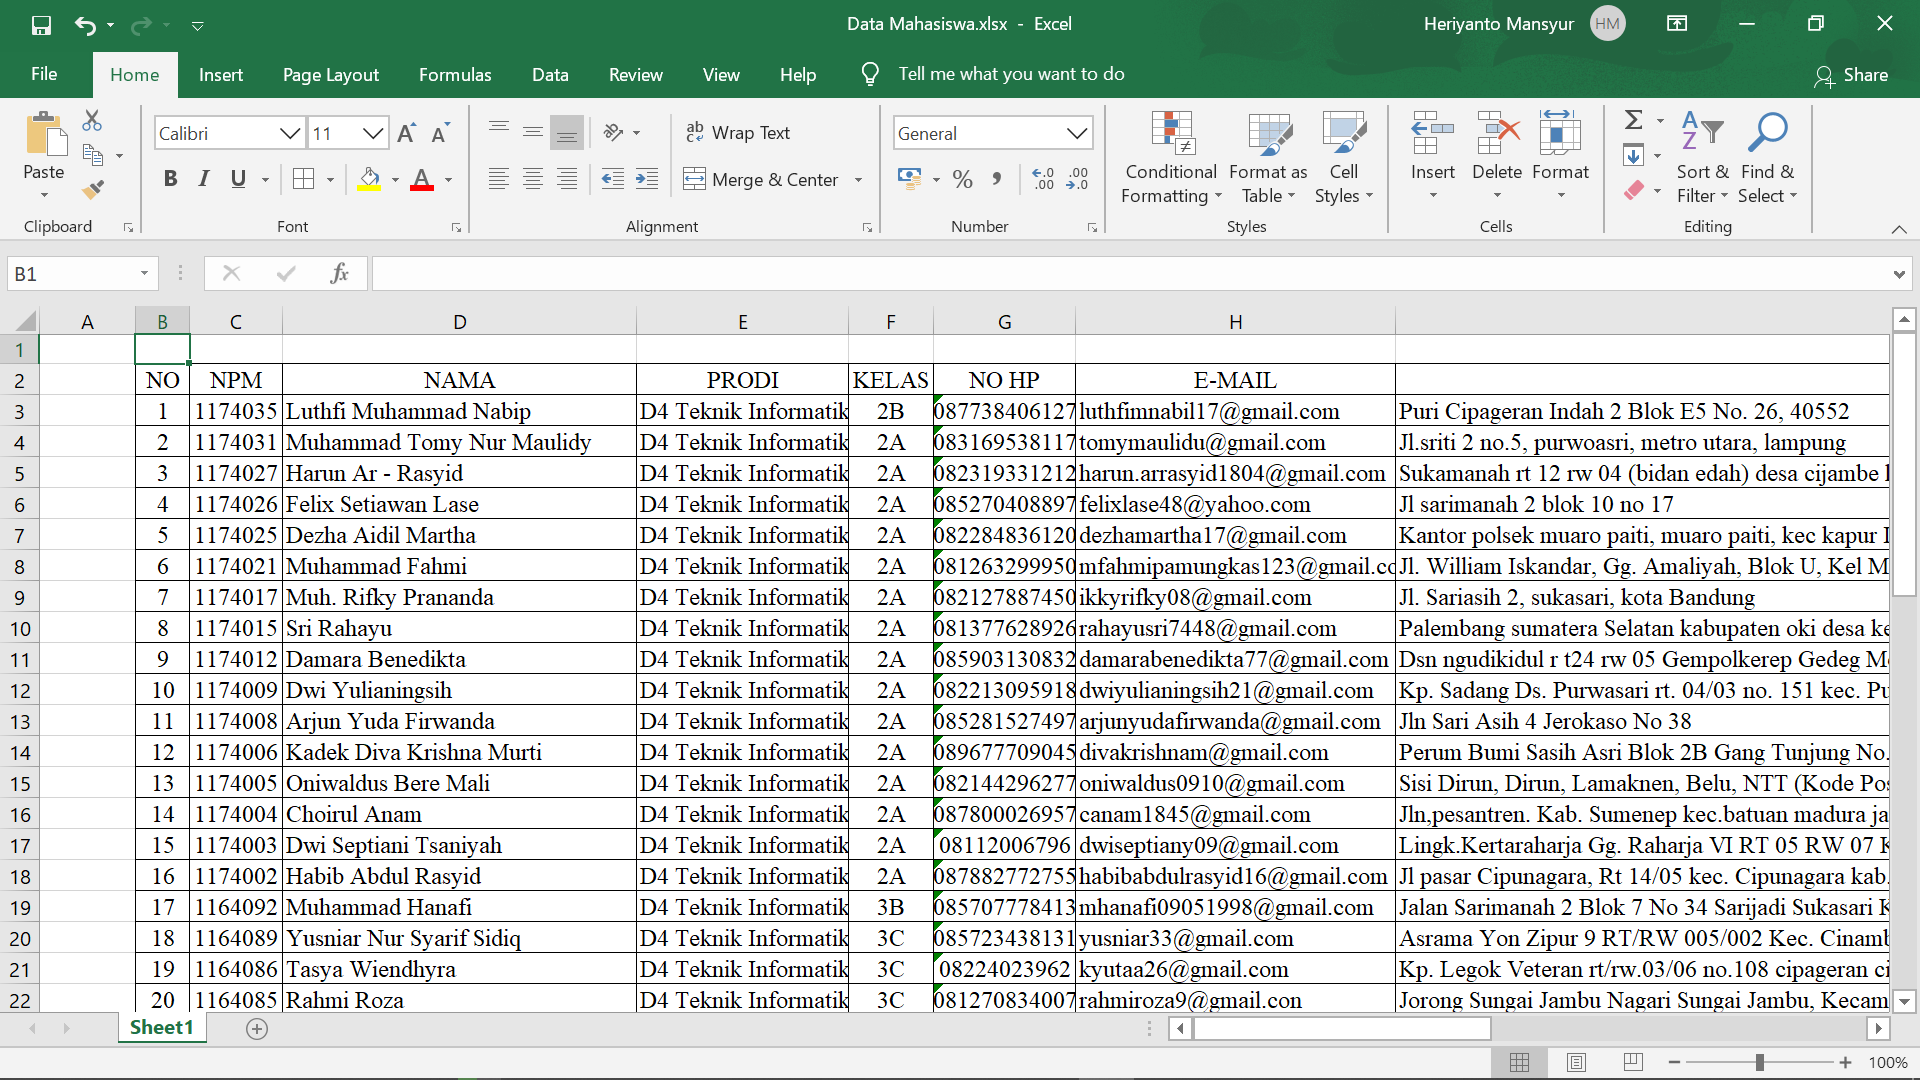
\includegraphics[width=10cm]{figures/1.png}
	\caption{File excel}
\end{figure}
\item Jika sudah ada, silahkan akses ke https://apex.oracle.com/pls/apex/, lalu masukkan workspace, username, dan password sesuai dengan yang anda miliki.
\begin{figure}[htbp]
	\centering
	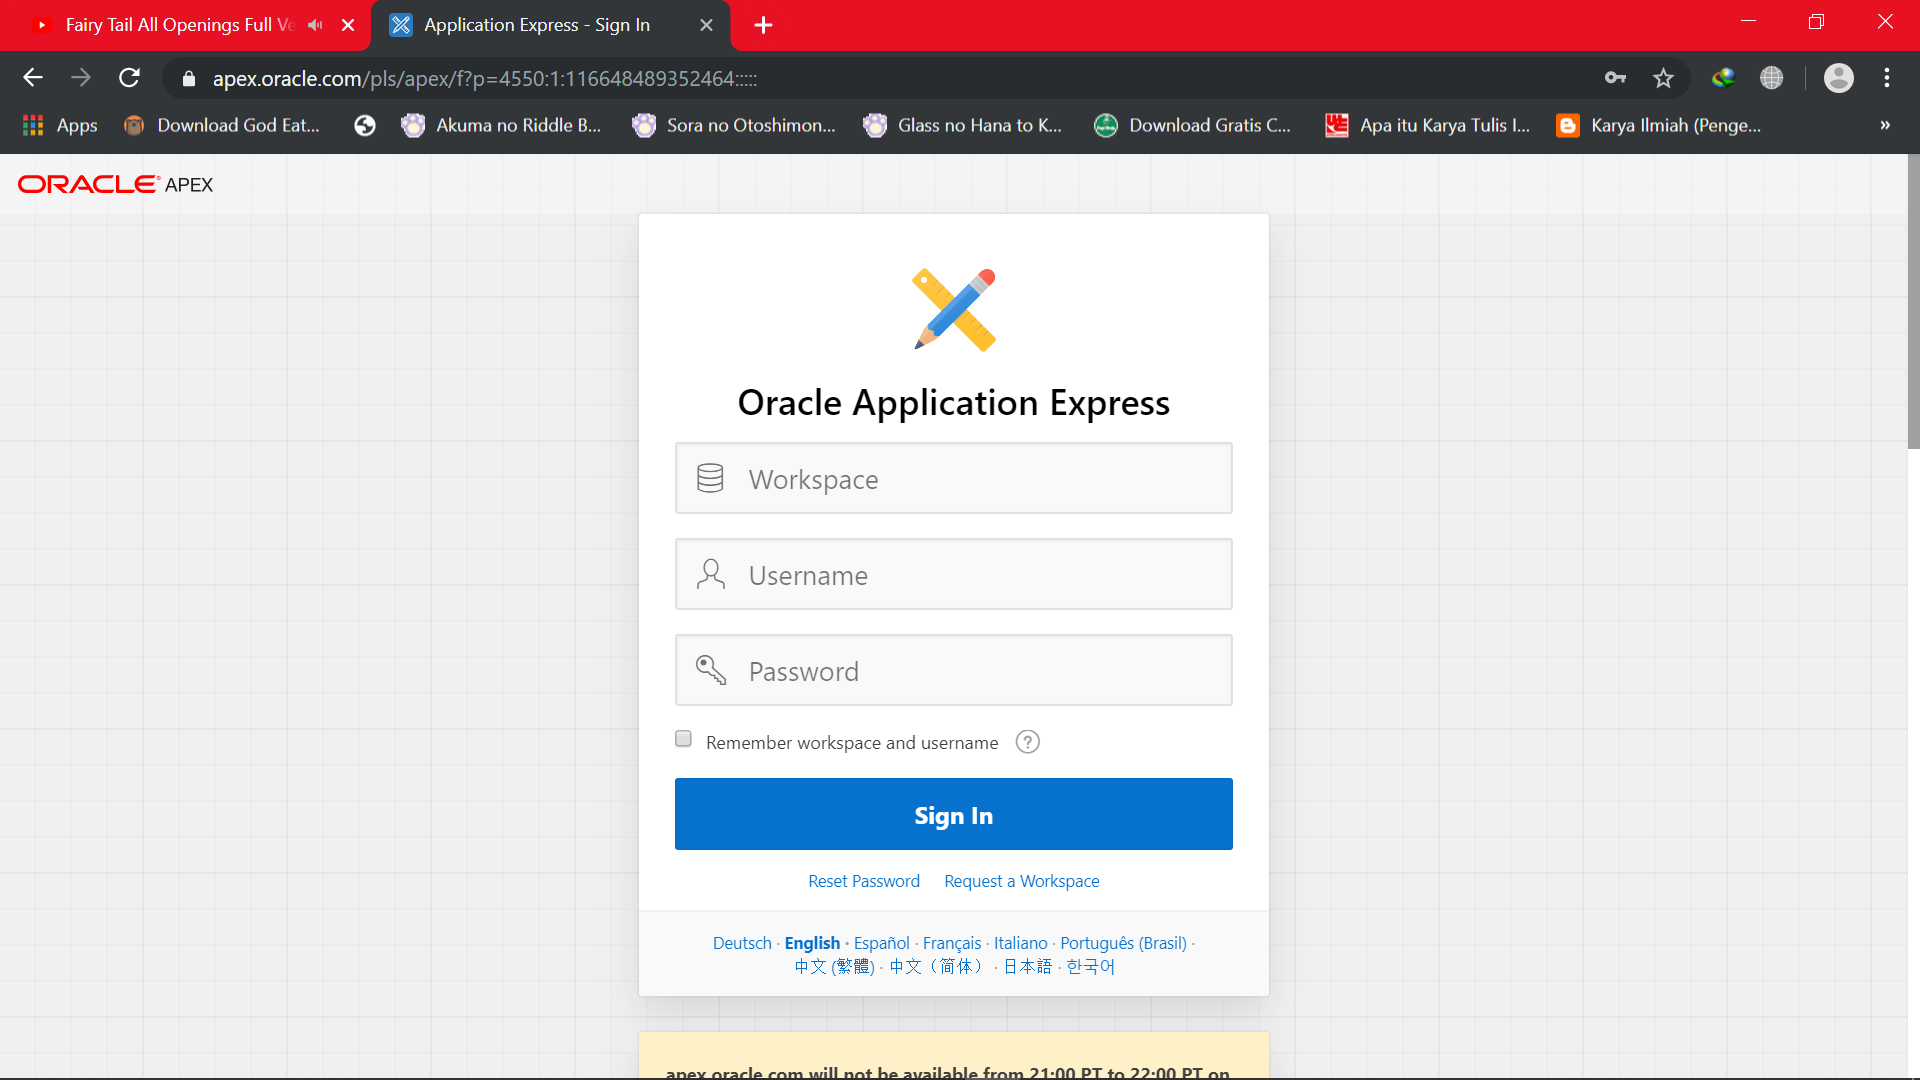
\includegraphics[width=10.5cm]{figures/2.png}
	\caption{Login ke Apex Oracle}
\end{figure}
\item Pada halaman utama apex oracle klik tombol "App Builder" untuk membuat aplikasi.
\begin{figure}[htbp]
	\centering
	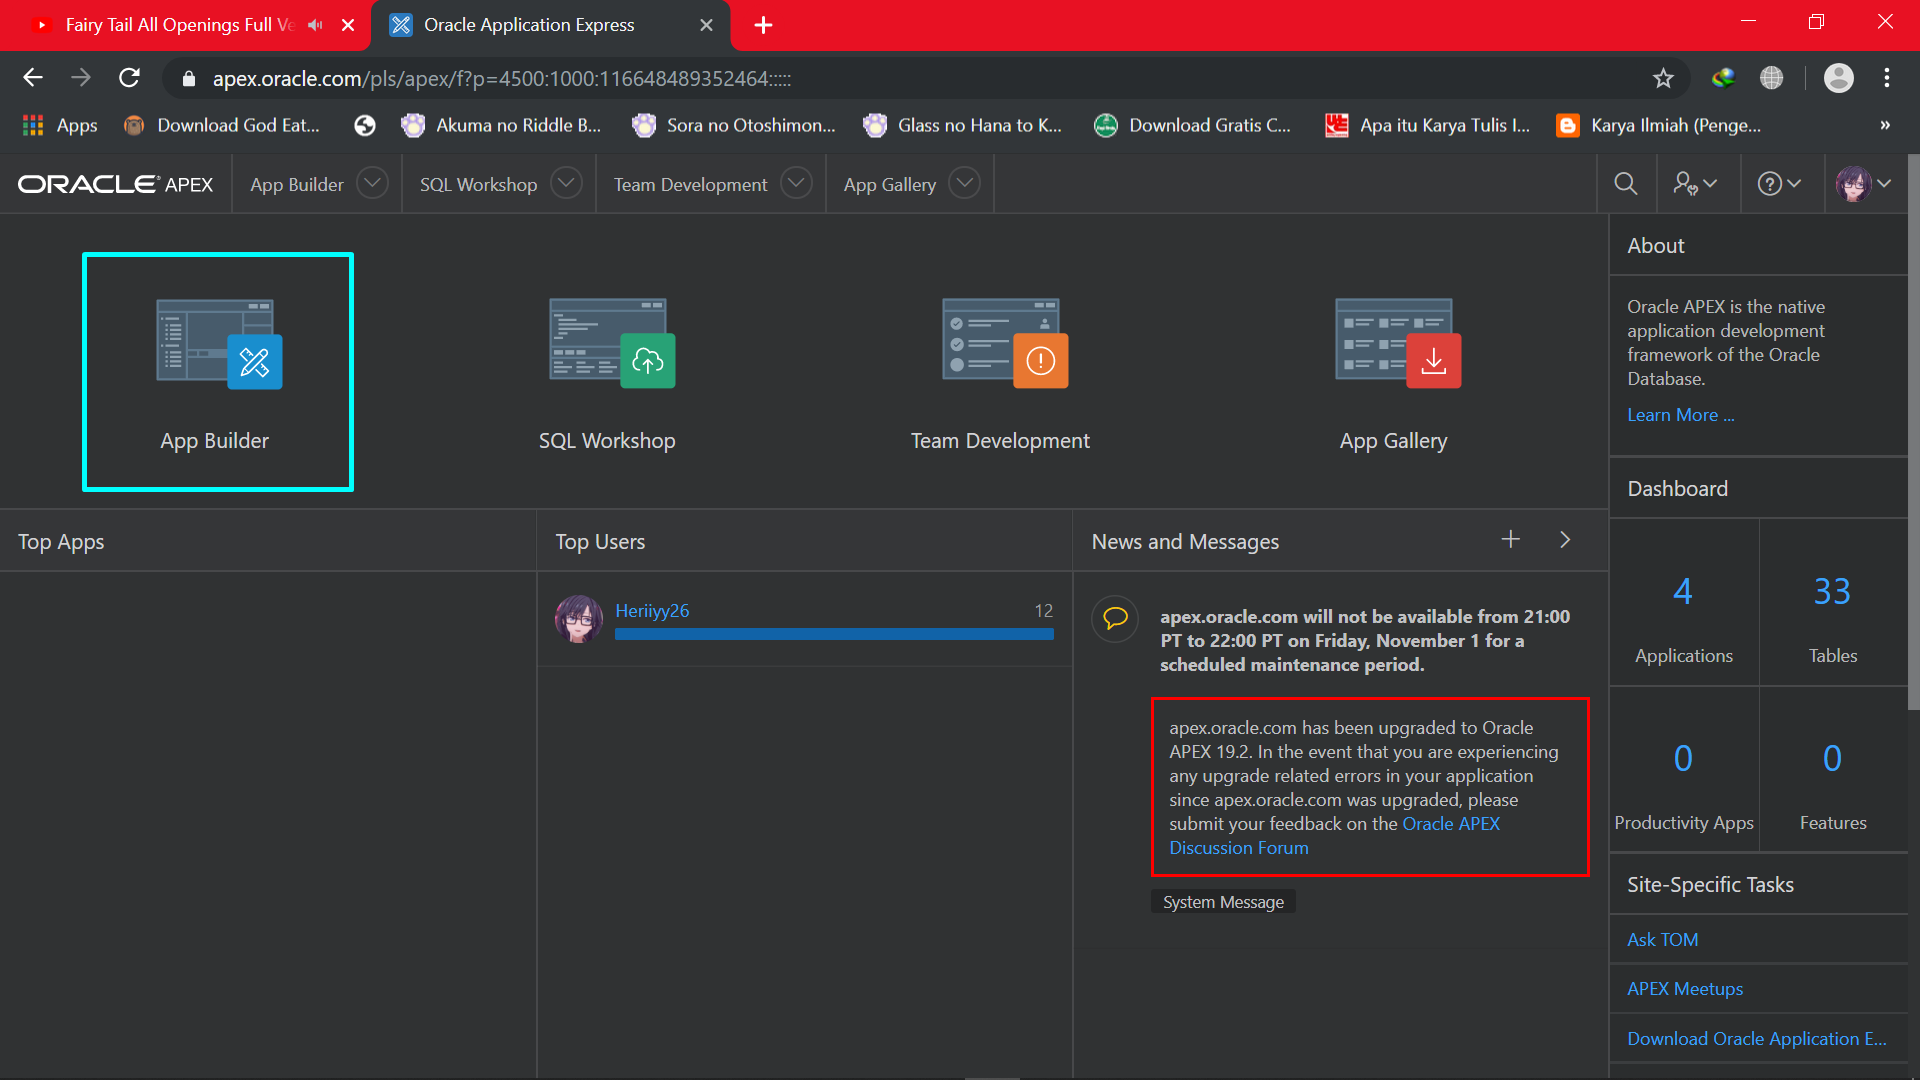
\includegraphics[width=10.5cm]{figures/3.png}
	\caption{Membuka App Builder}
\end{figure}\\
\\
\item Pada halaman App Builder klik tombol "Create" untuk memulai membuat aplikasi.
\begin{figure}[htbp]
	\centering
	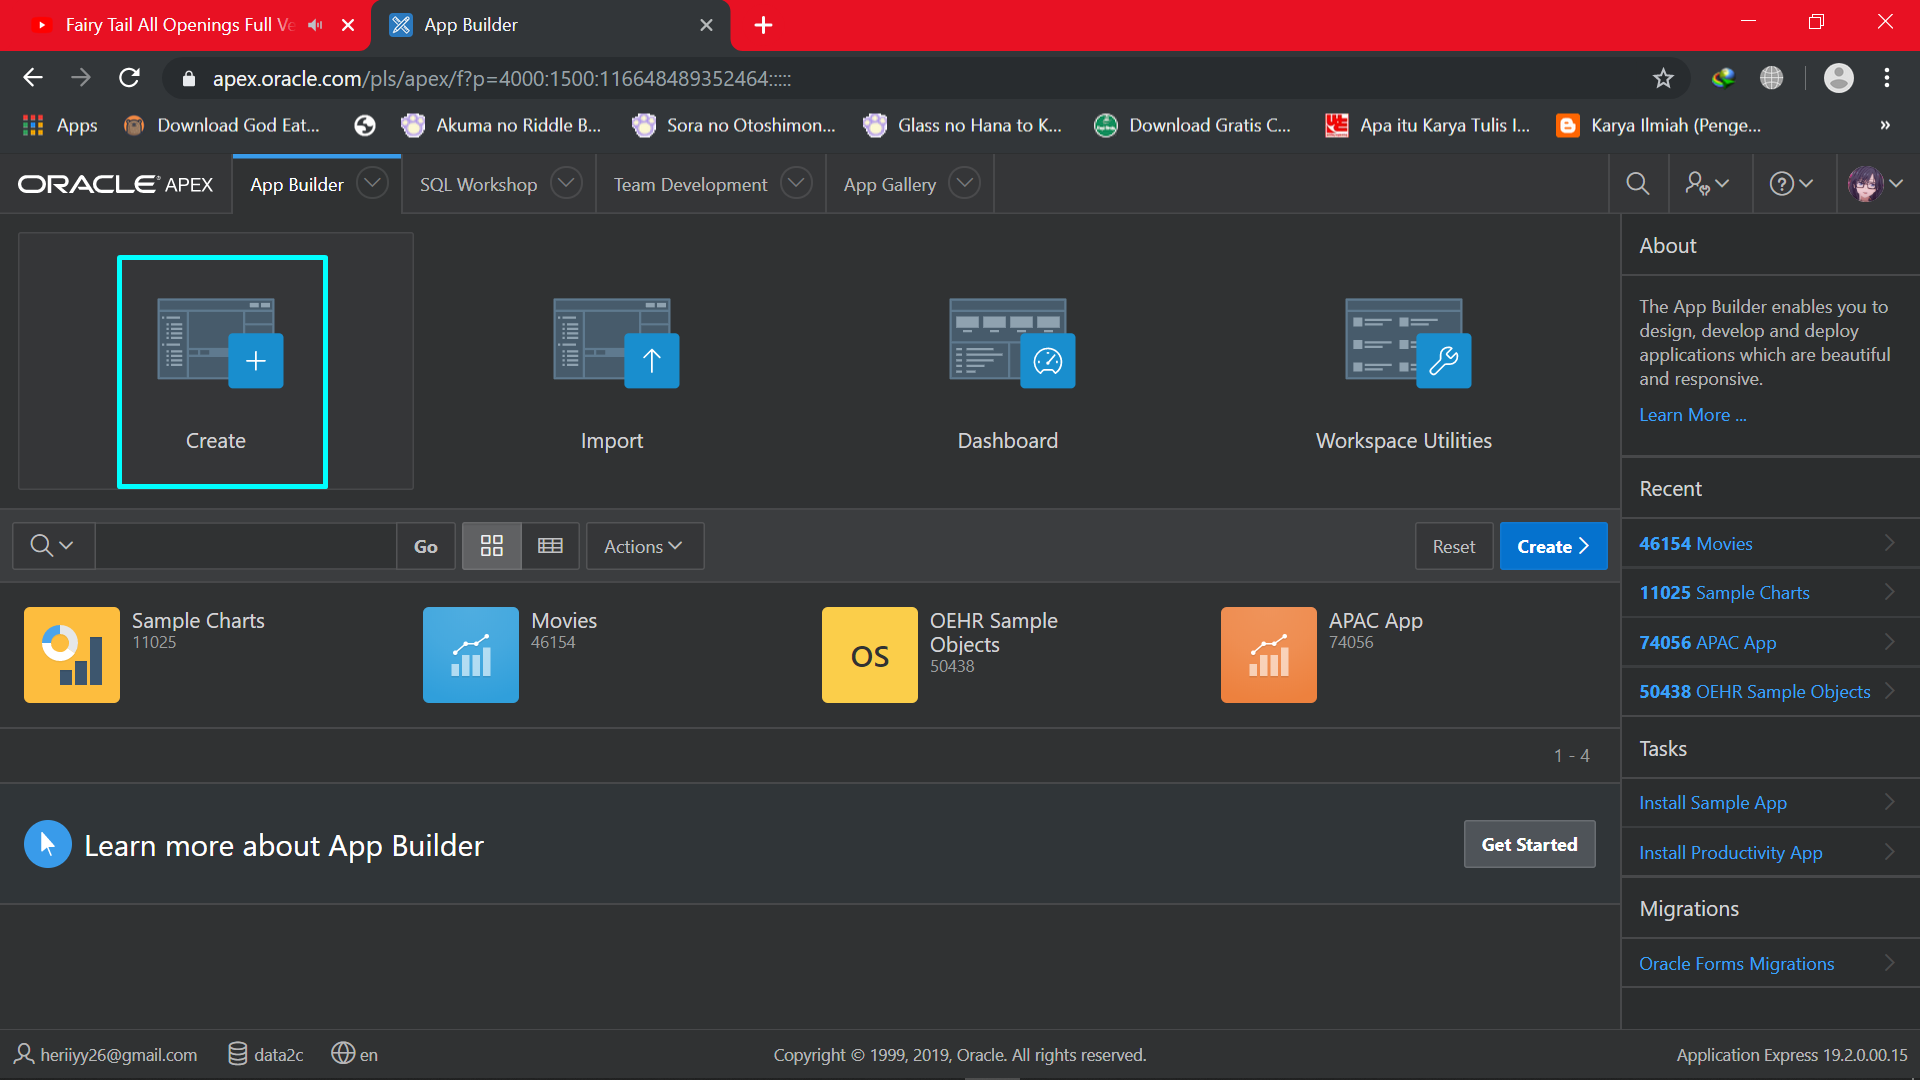
\includegraphics[width=10.5cm]{figures/4.png}
	\caption{Memulai membuat Aplikasi}
\end{figure}
\item Pada halaman Create Application ada tiga fitur dalam membuat aplikasi, disini kita akan memakai fitur "From a File" dari file excel kita tadi, jadi silahkan klik.
\begin{figure}[htbp]
	\centering
	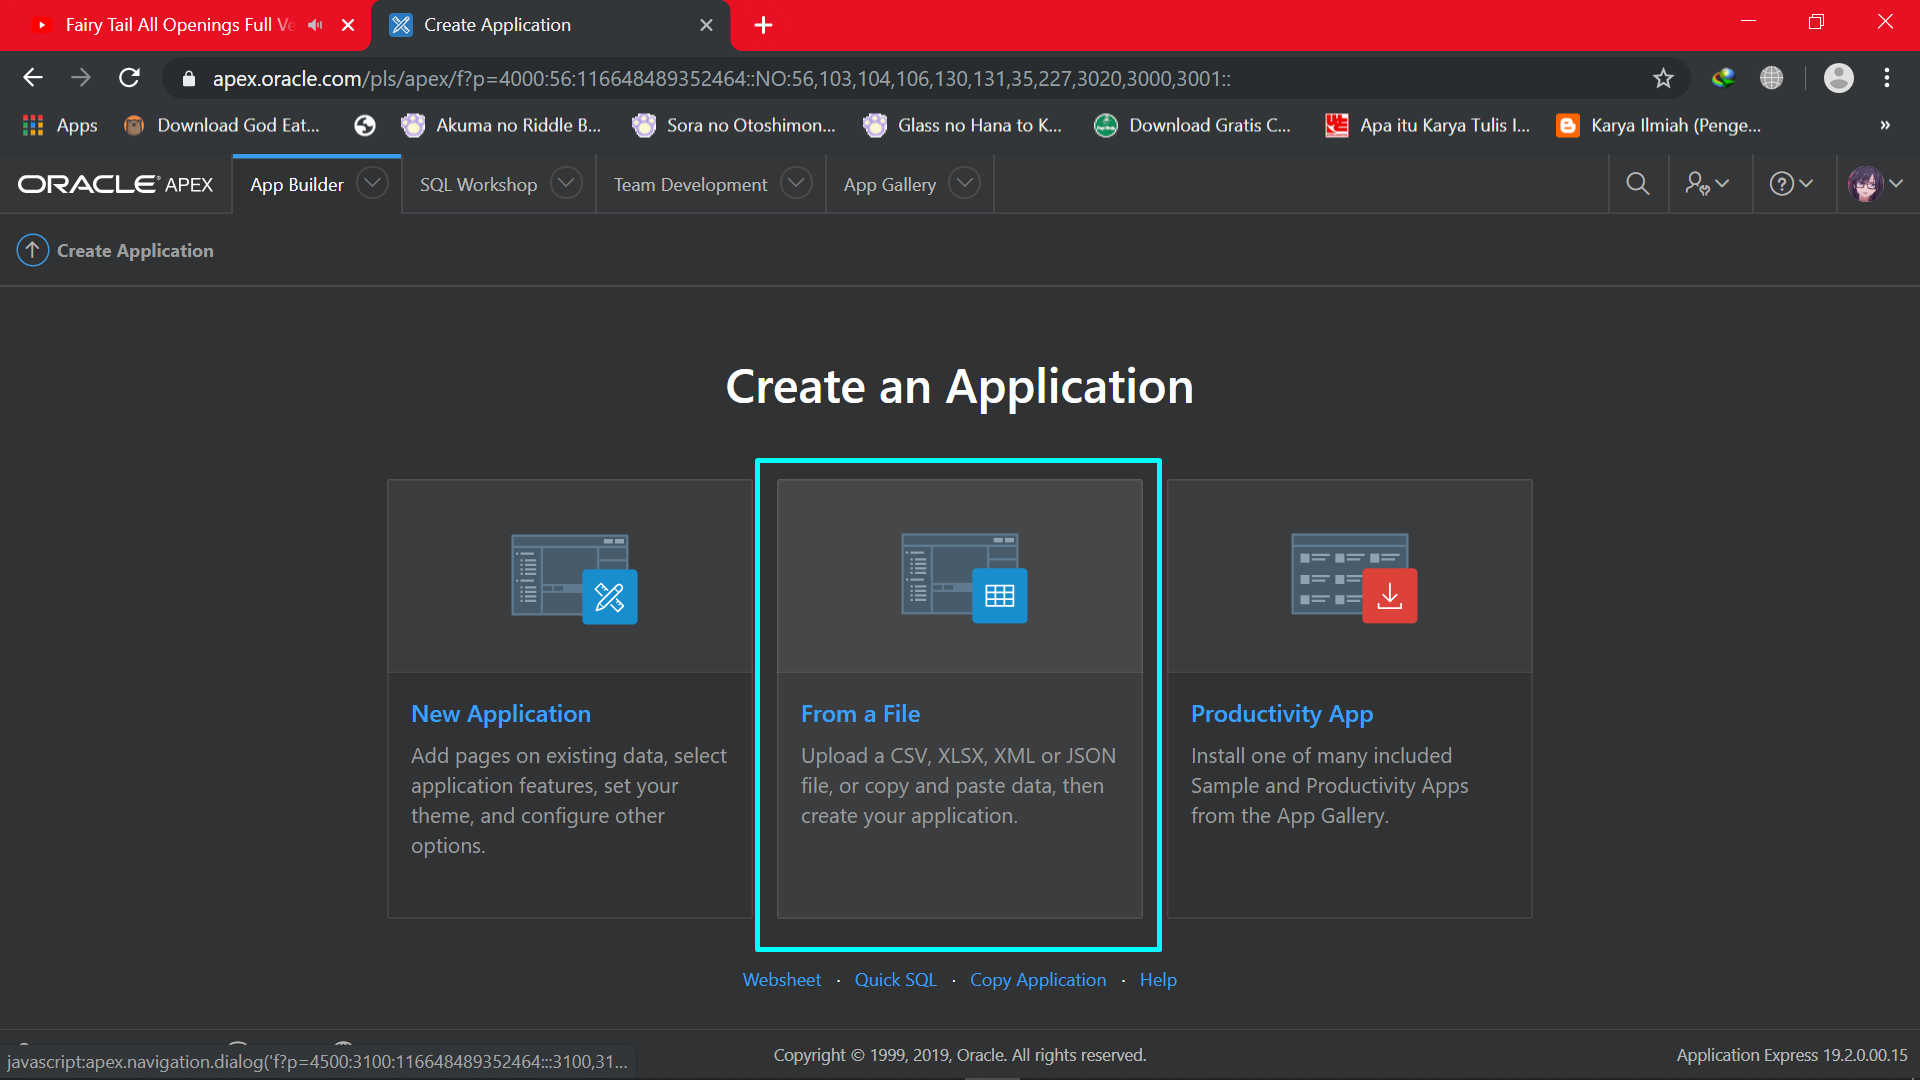
\includegraphics[width=10.5cm]{figures/5.png}
	\caption{Membuat aplikasi dari file}
\end{figure}\\
\\
\item Setelah di-klik akan muncul dialog load data, di dialog tersebut pilih tab "Upload a File" lalu klik tombol "Choose File".
\begin{figure}[htbp]
	\centering
	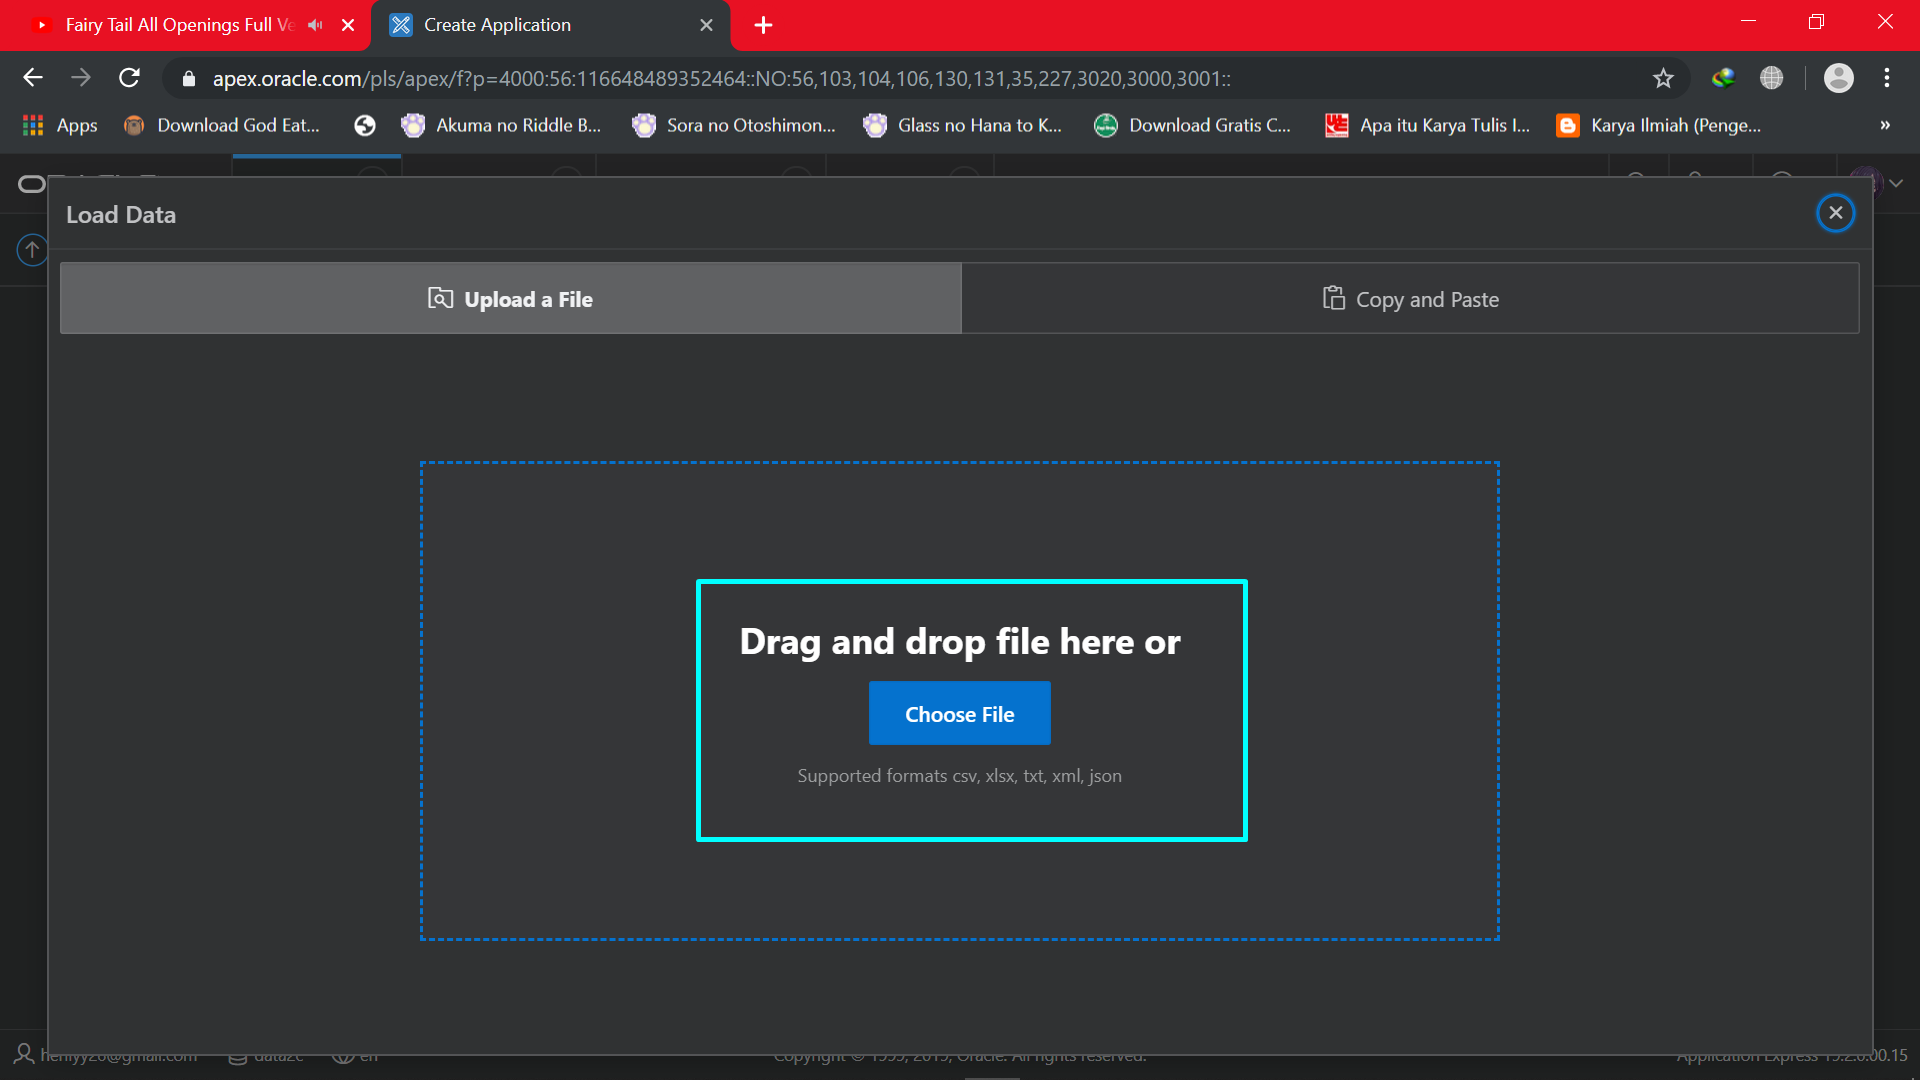
\includegraphics[width=10.5cm]{figures/6.png}
	\caption{Meng-upload file}
\end{figure}
\item Buka tempat dimana file excel anda tersimpan, disini file saya adalah Data Mahasiswa.xlsx.
\begin{figure}[htbp]
	\centering
	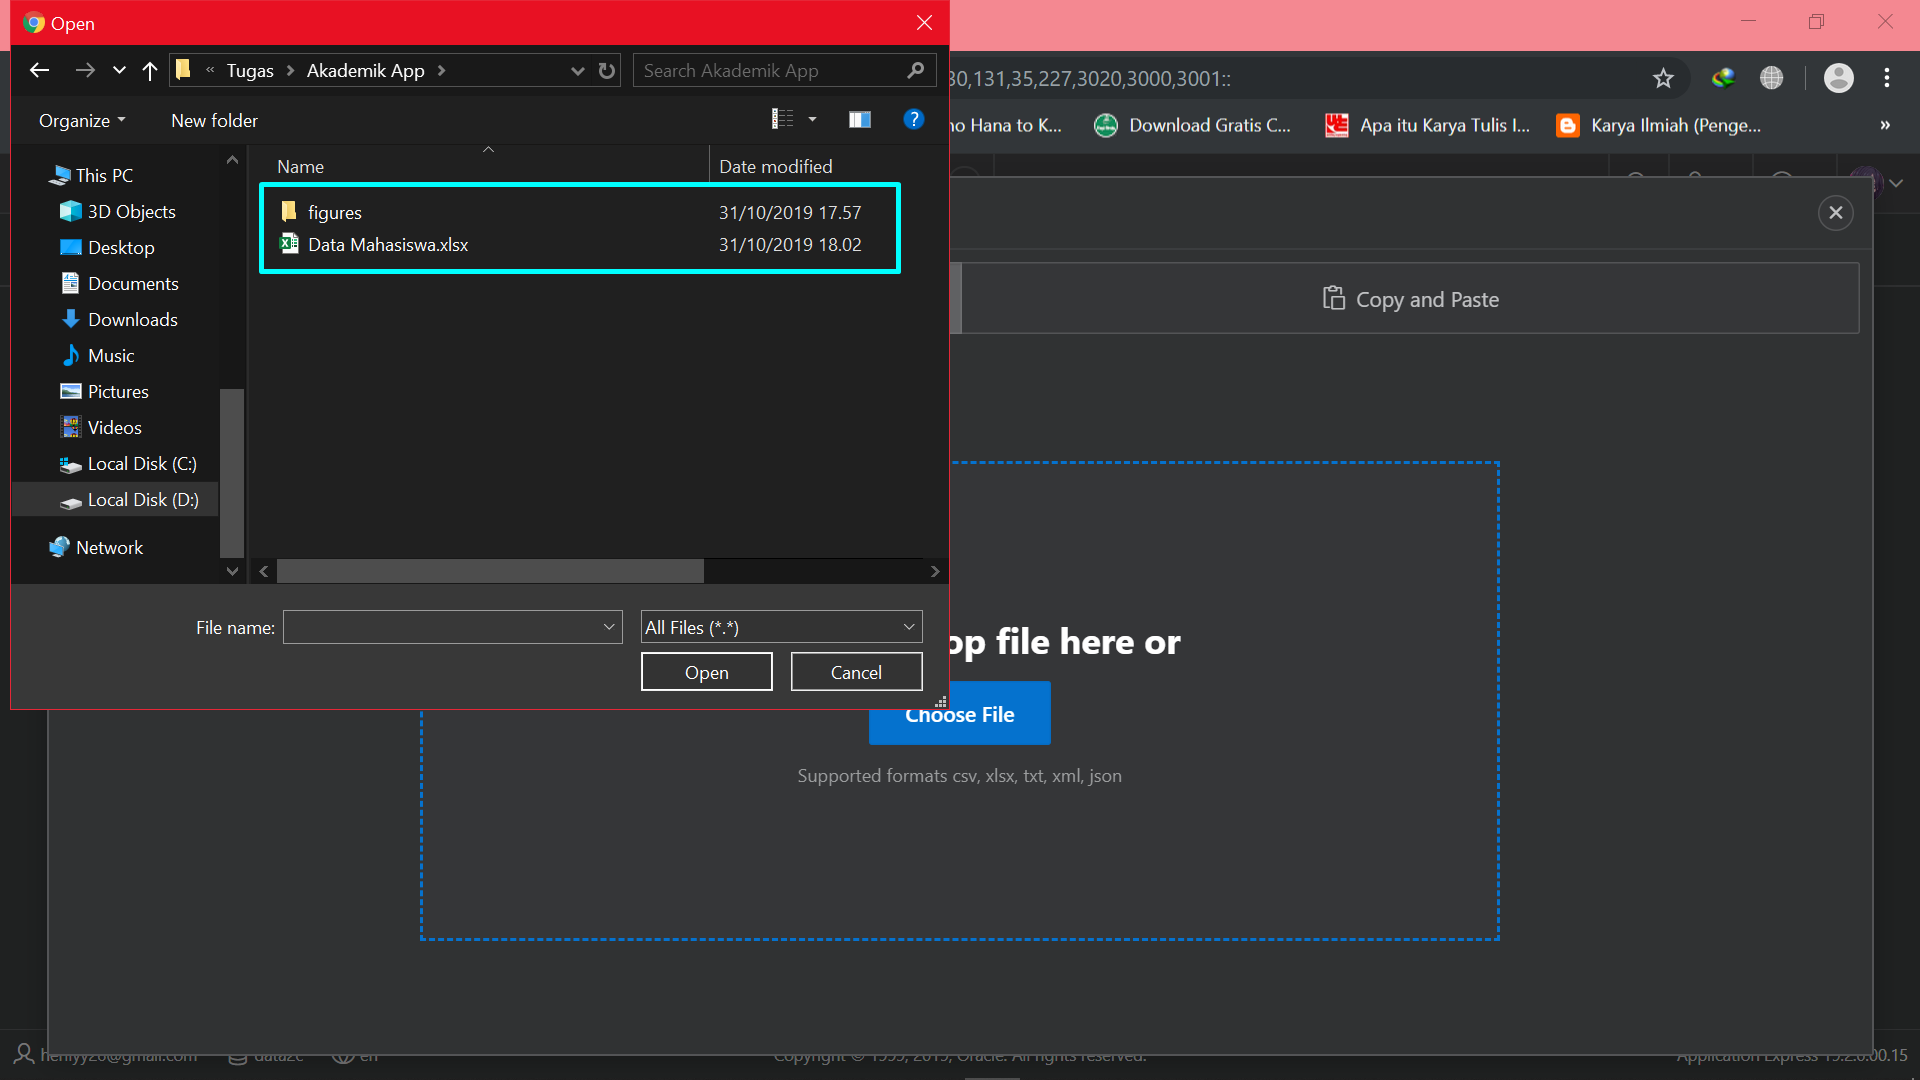
\includegraphics[width=10.5cm]{figures/7.png}
	\caption{Membuka tempat file disimpan}
\end{figure}\\
\\
\item JIka sudah silahkan isi nama tabel dengan nama "Mahasiswa", lalu klik "Load Data". 
\begin{figure}[htbp]
	\centering
	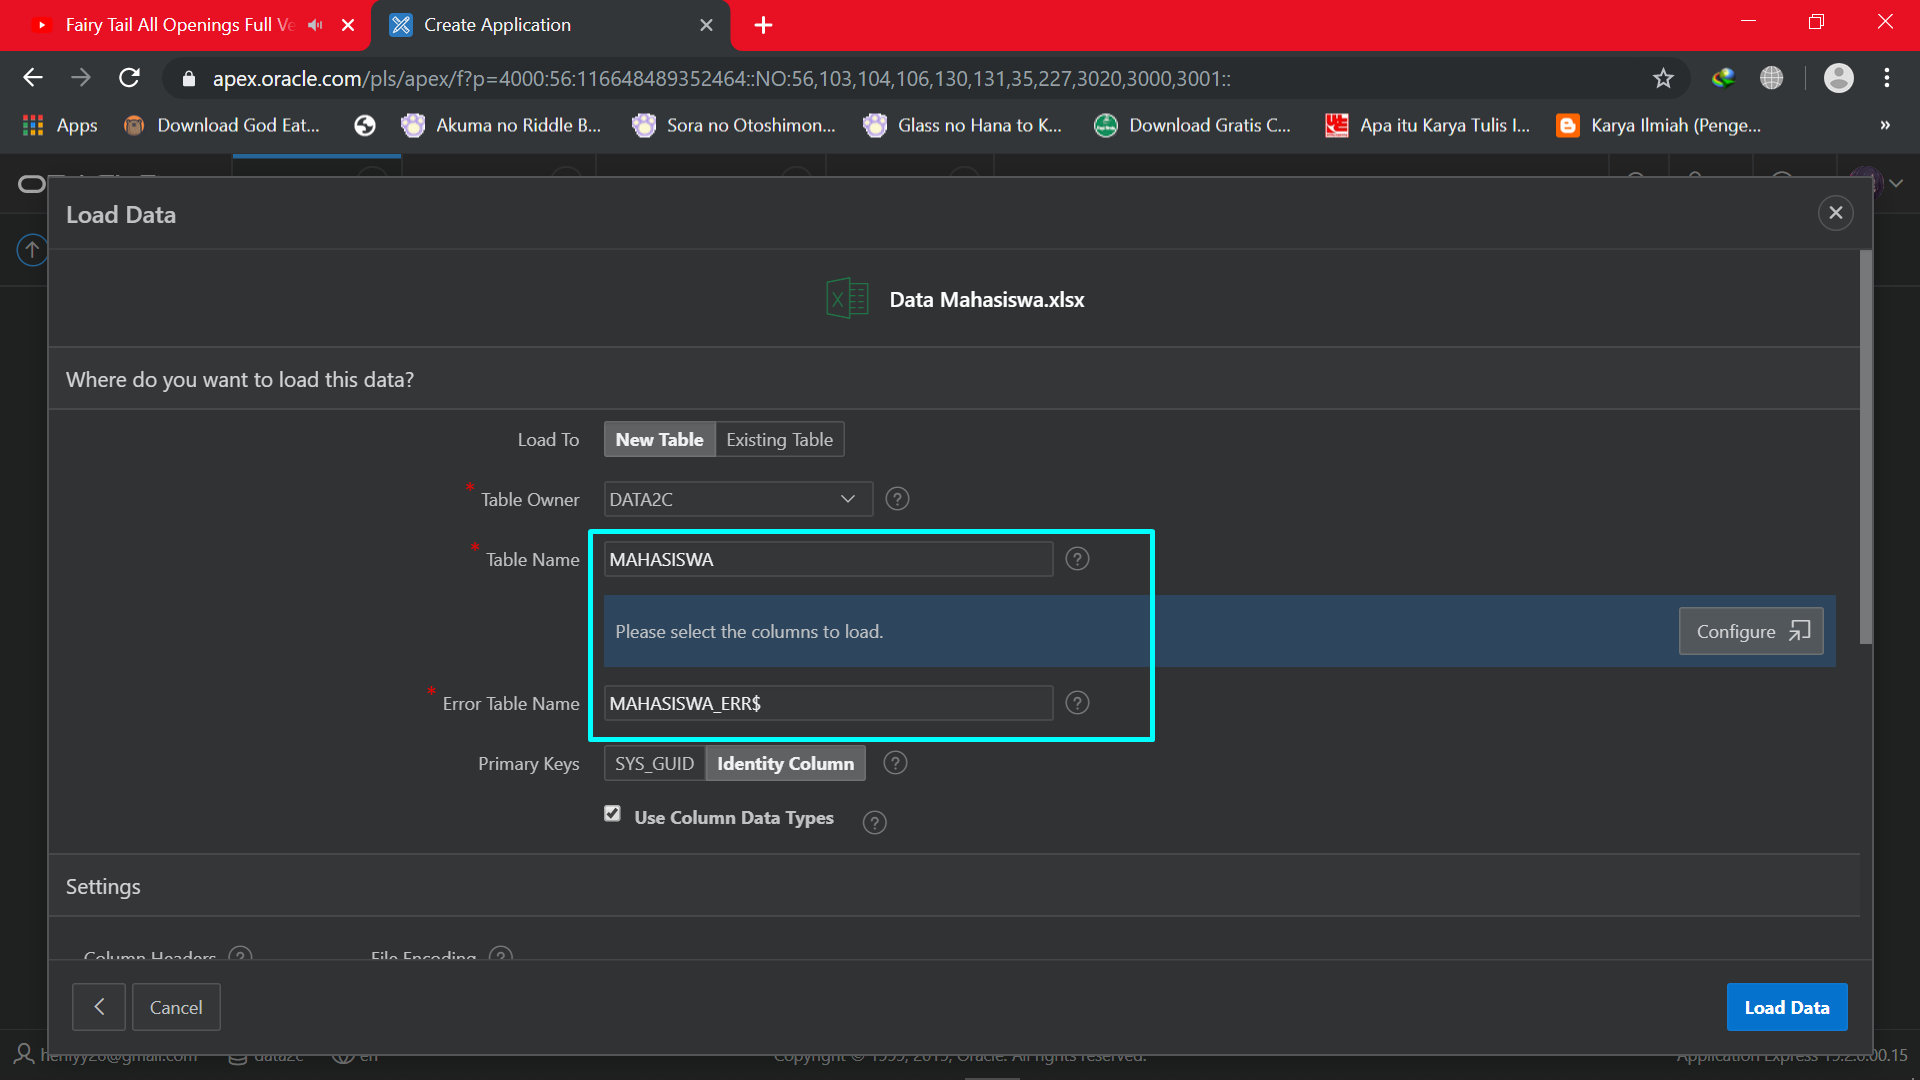
\includegraphics[width=10.5cm]{figures/8.png}
	\caption{Memberi nama tabel}
\end{figure}
\item Load Data sukses, klik "view table" untuk memastikan tabel mahasiswa sudah bernar.
\begin{figure}[htbp]
	\centering
	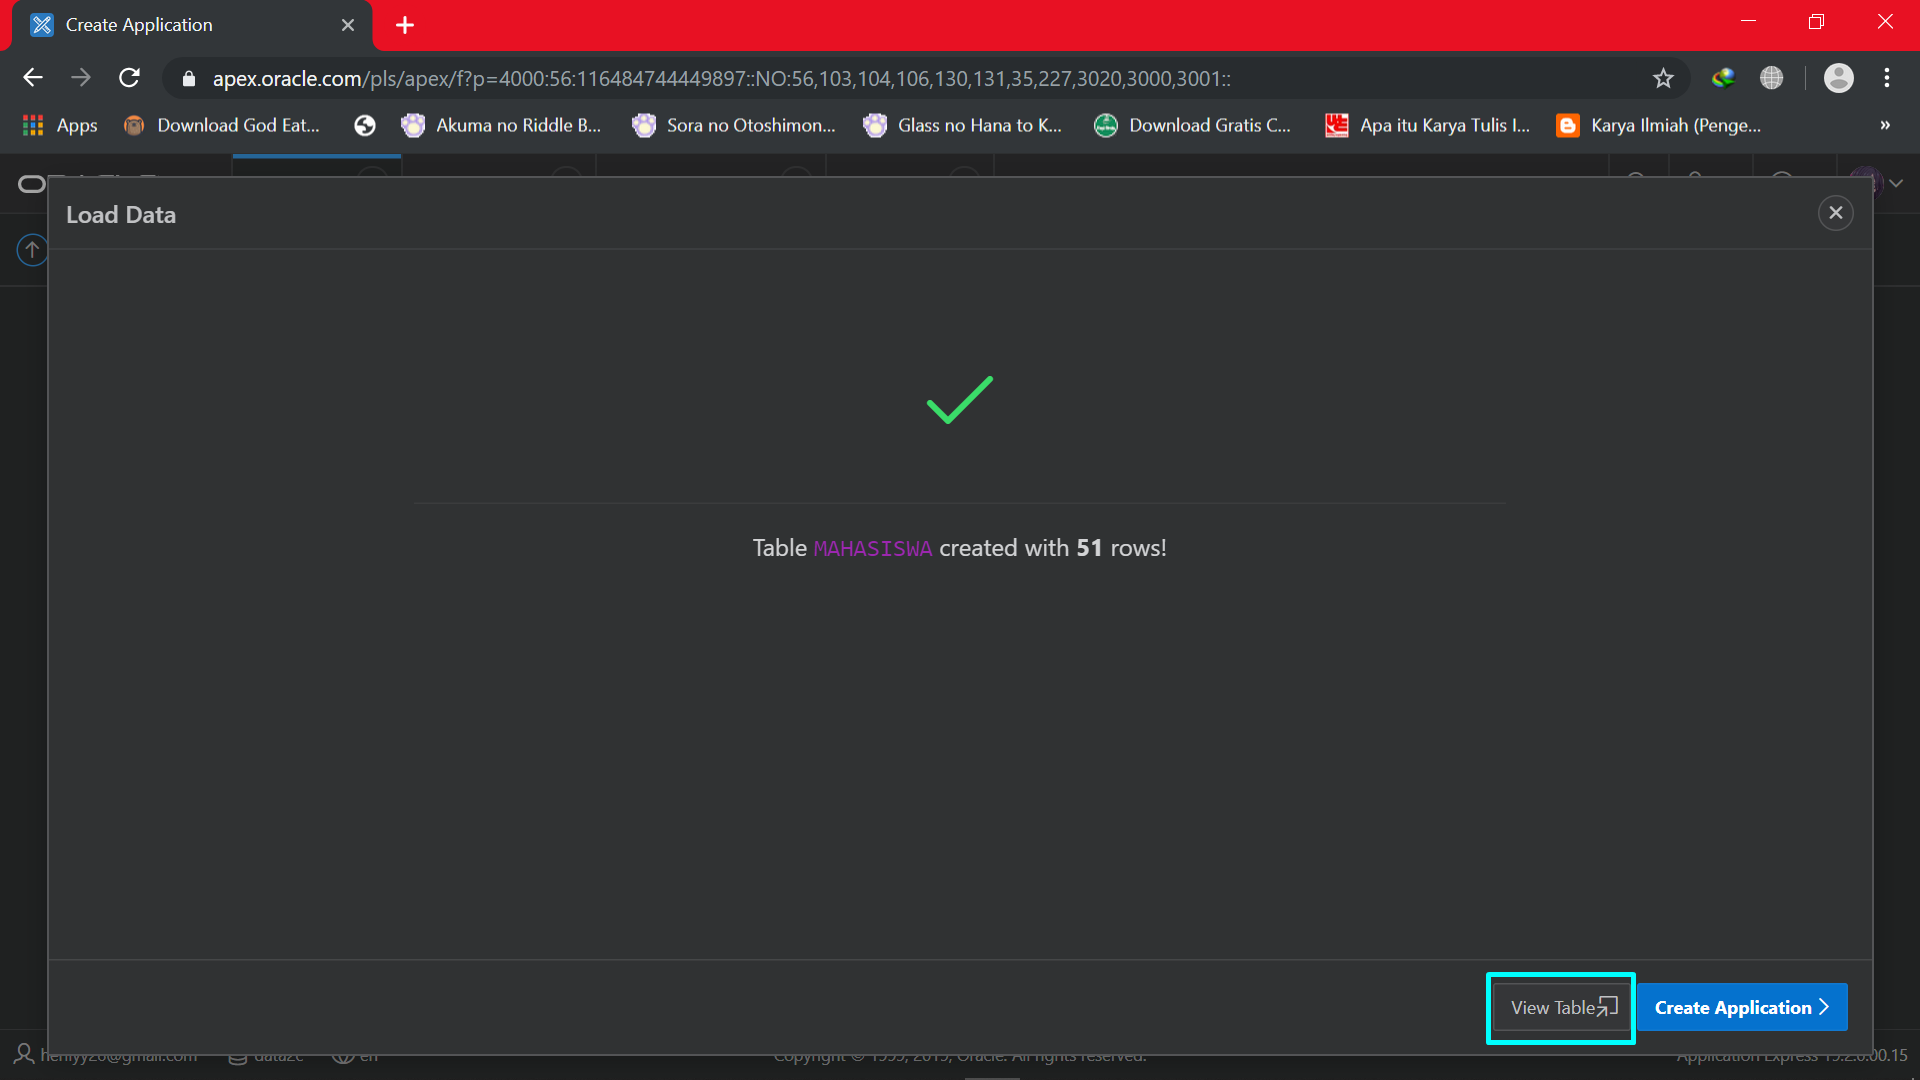
\includegraphics[width=10.5cm]{figures/9.png}
	\caption{Load Data}
\end{figure}\\
\\
\item Bisa dilihat pada gambar di bawah bahwa tabel mahasiswa masih belum benar, ada kolom yang tidak berisi data, nama kolom tidak jelas, dan ada data yang tidak sesuai, maka dari kita akan normalisasi tabel tersebut.
\begin{figure}[htbp]
	\centering
	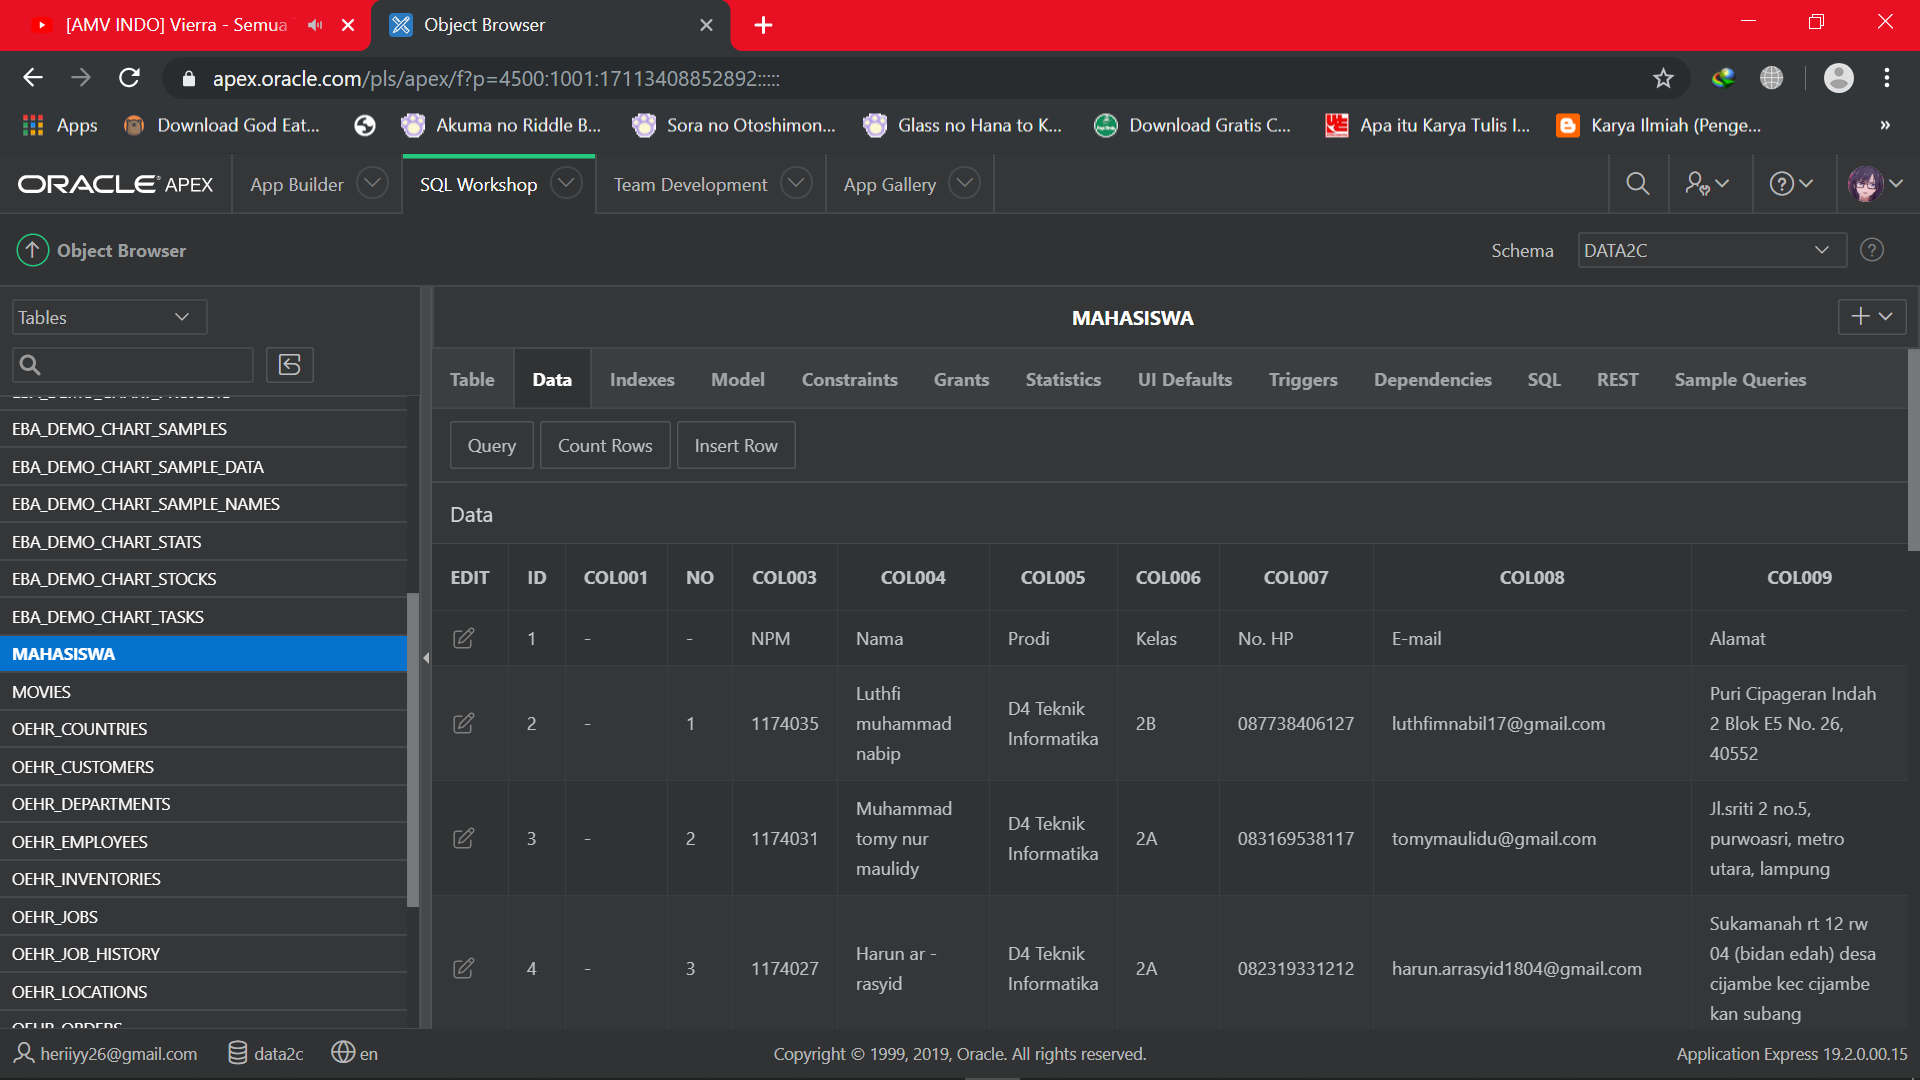
\includegraphics[width=10cm]{figures/10.png}
	\caption{Tabel Mahasiswa}
\end{figure}
\item Yang pertama adalah drop kolom "COL001" dan kolom "NO", caranya adalah klik pada tab "Table" lalu pilih "Drop Column".
\begin{figure}[htbp]
	\centering
	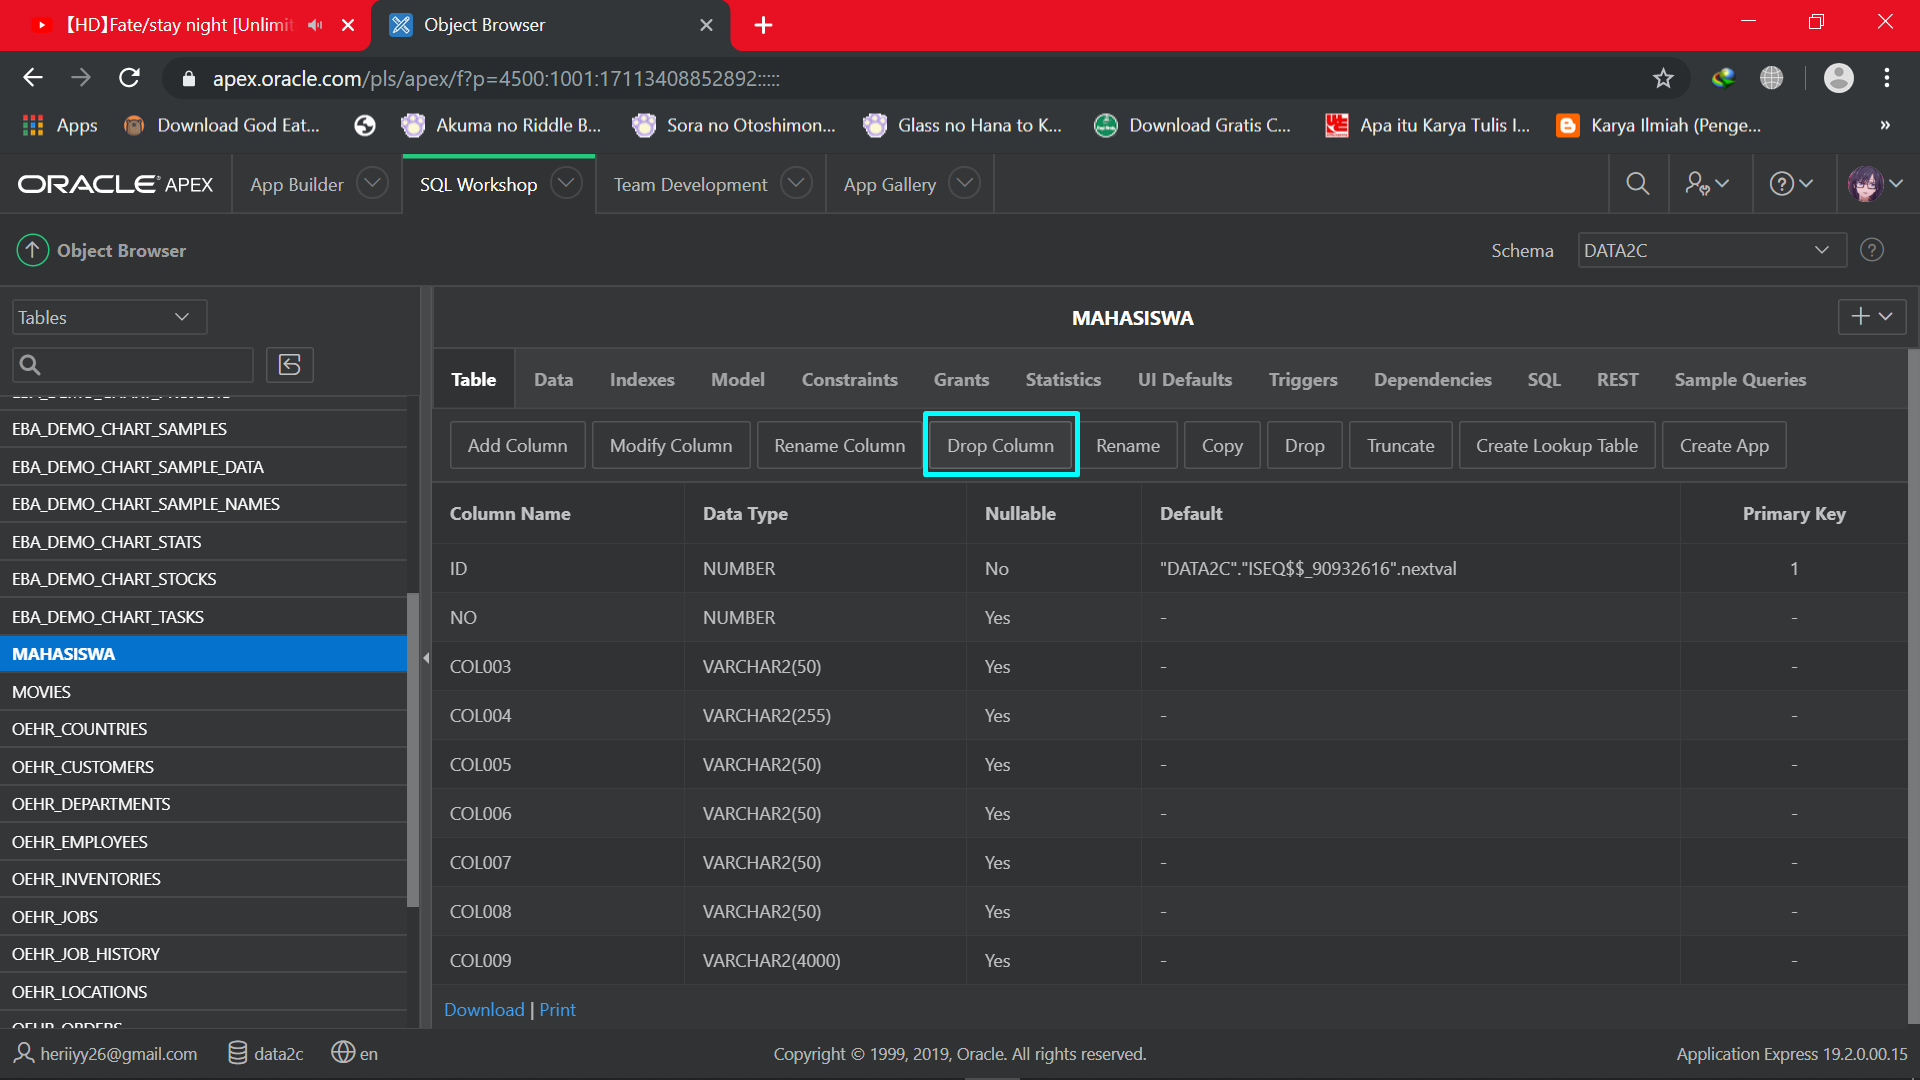
\includegraphics[width=10cm]{figures/11.png}
	\caption{Drop Column}
\end{figure}
\item Selanjutnya akan dialihkan ke halaman Drop Column, di halaman pilih kolom yang ingin di hapus, yaitu kolom "NO" di list "-Select Column-" lalu klik "Next".
\begin{figure}[htbp]
	\centering
	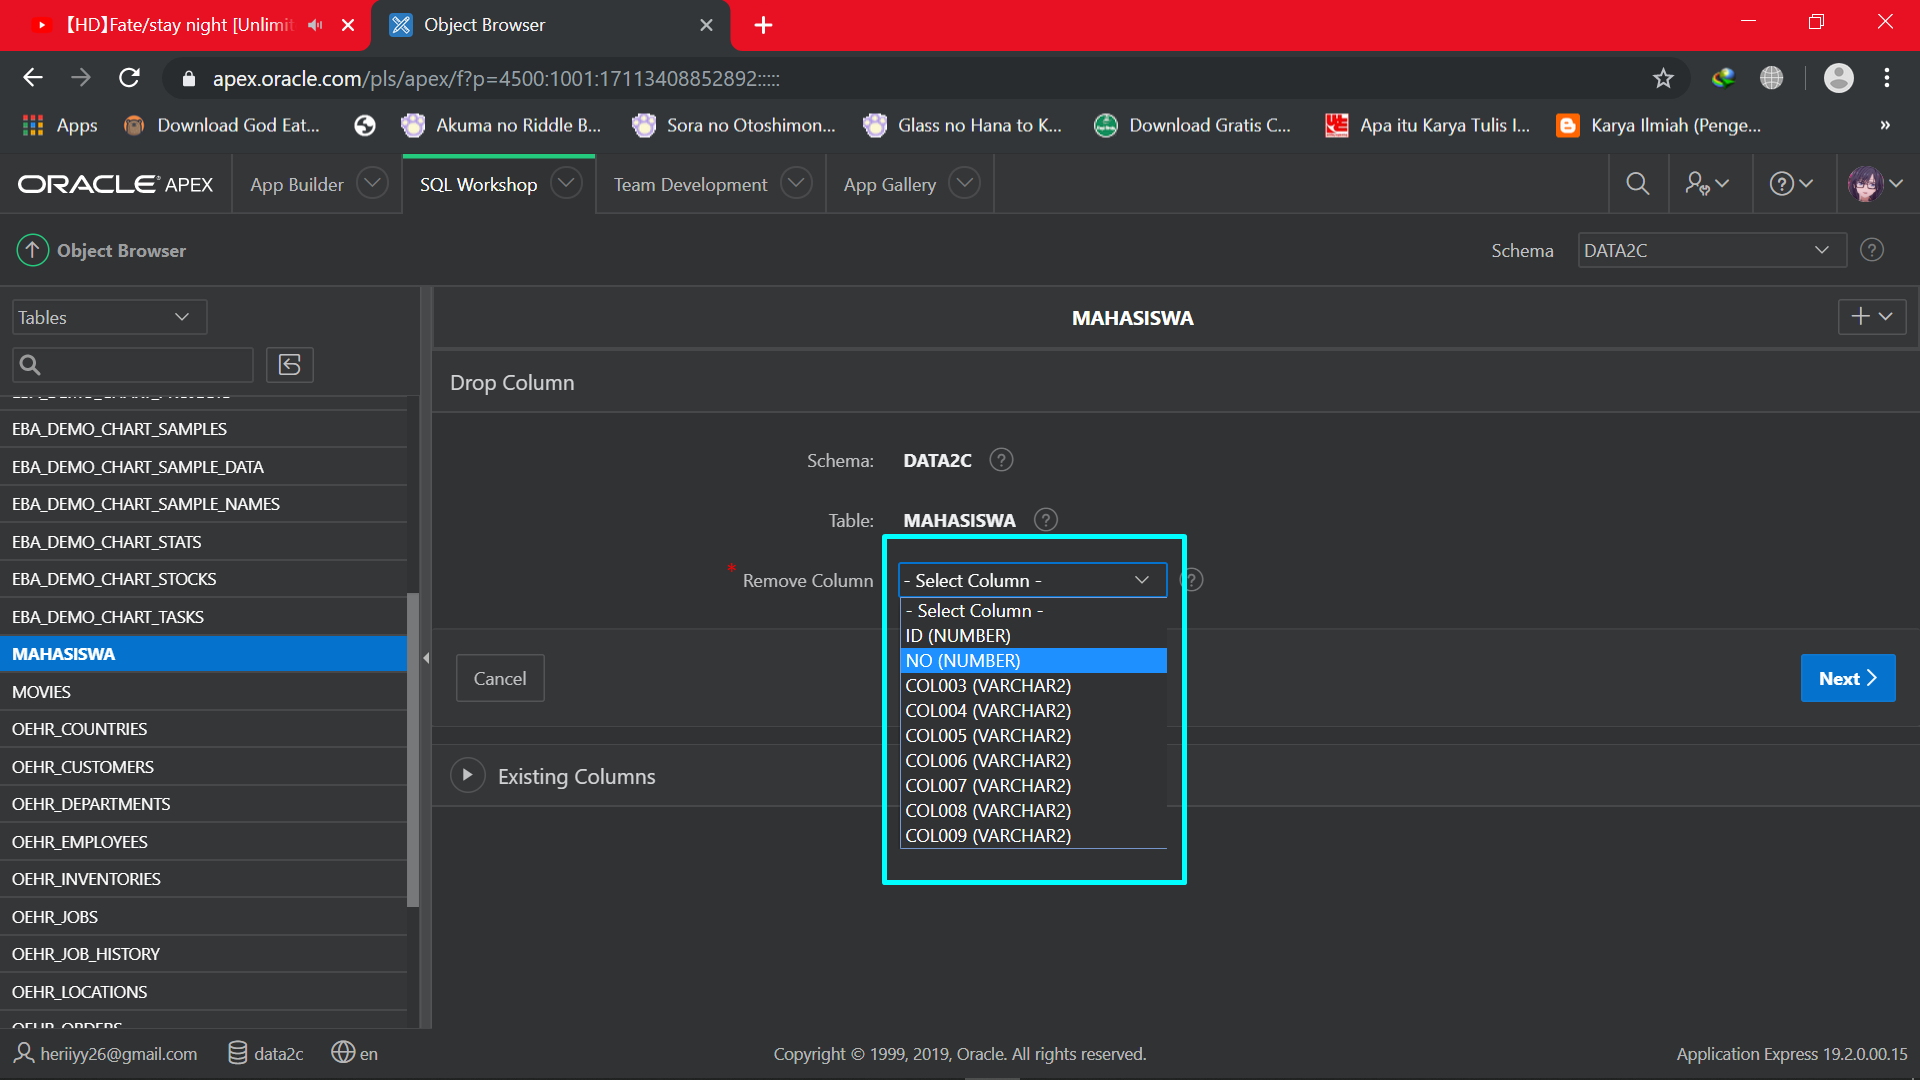
\includegraphics[width=10cm]{figures/12.png}
	\caption{Memilih kolom yang ingin dihapus}
\end{figure}
\item Selanjutnya akan dialihkan ke halaman Confirm, klik "Finish" untuk menghapus kolom yang dipilih tadi dan selesai, lakukan hal yang sama pada kolom "COL001".
\begin{figure}[htbp]
	\centering
	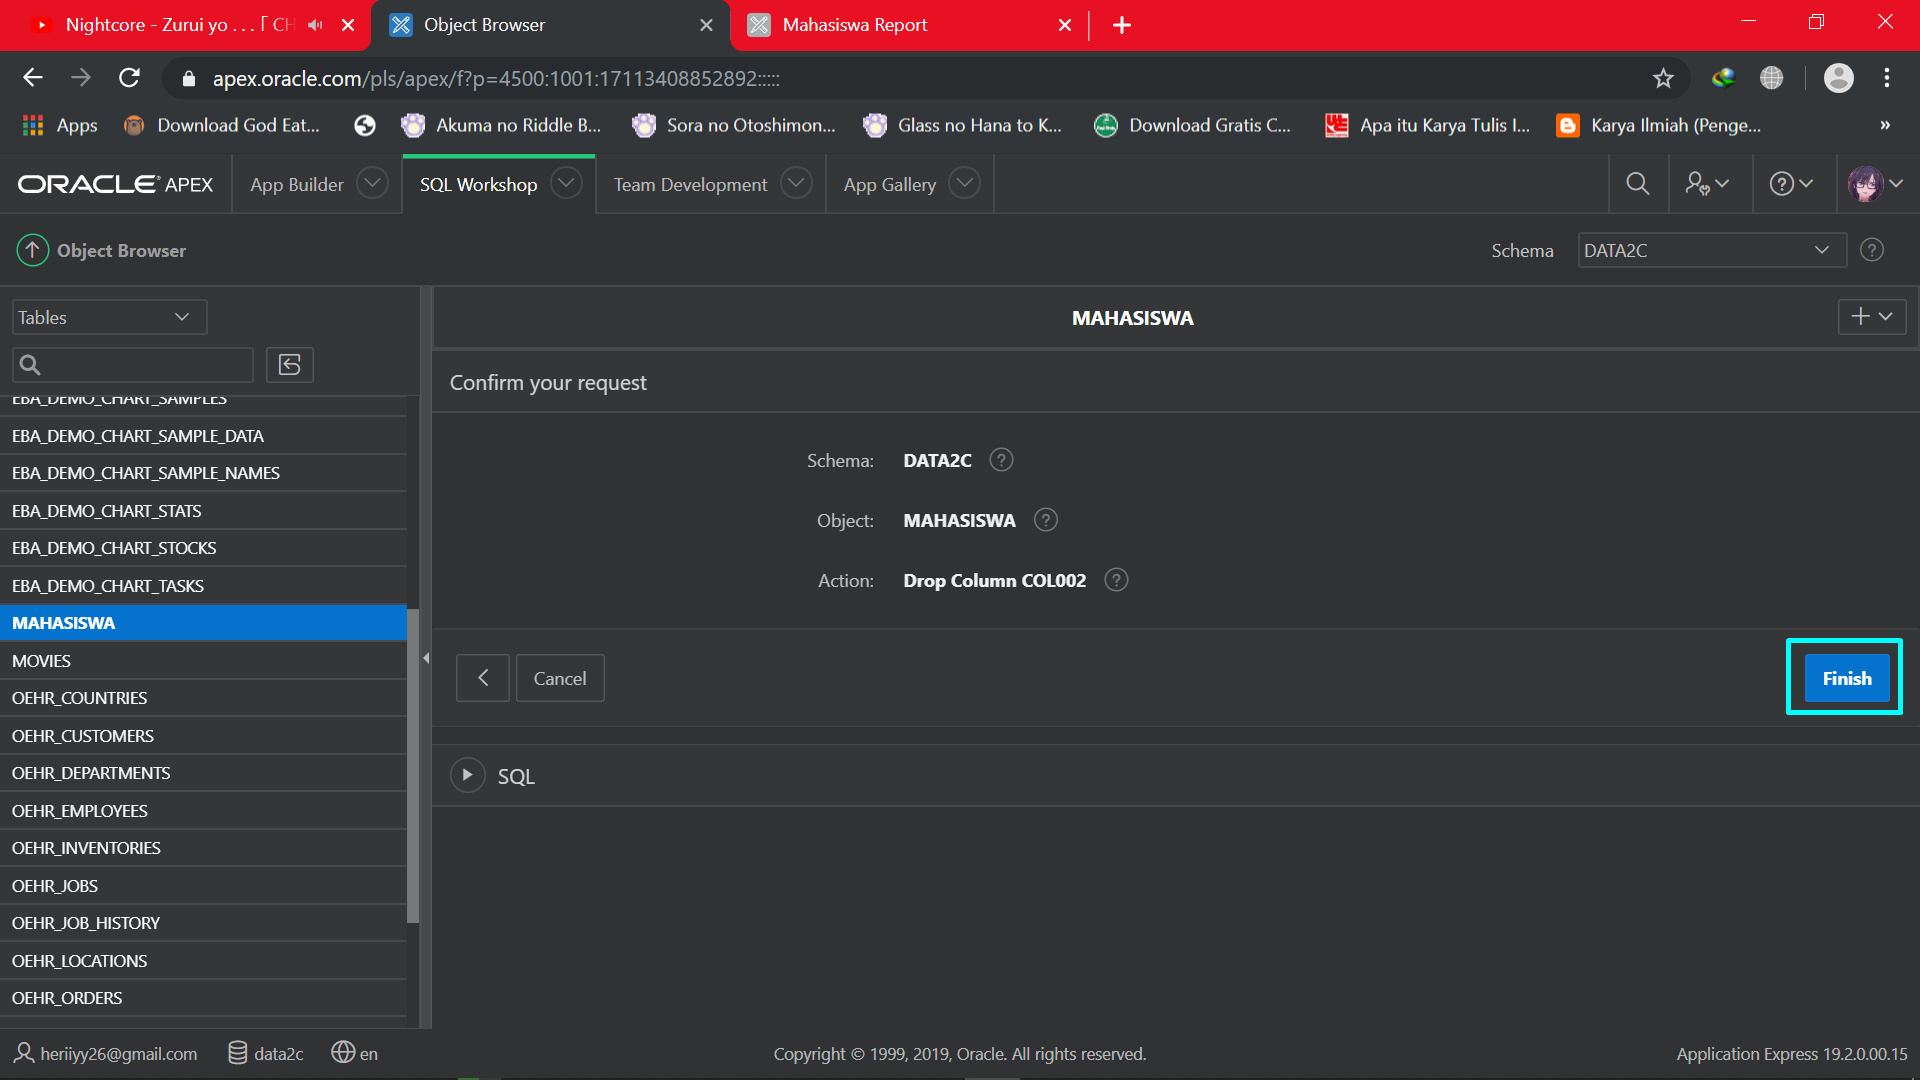
\includegraphics[width=10cm]{figures/13.png}
	\caption{Konfirmasi Kolom yang dihapus}
\end{figure}
\item Selanjutnya adalah mengganti nama kolom yang ada sesuai dengan data pada tabel. Caranya adalah klik "Rename Column" pada tab Table.
\begin{figure}[htbp]
	\centering
	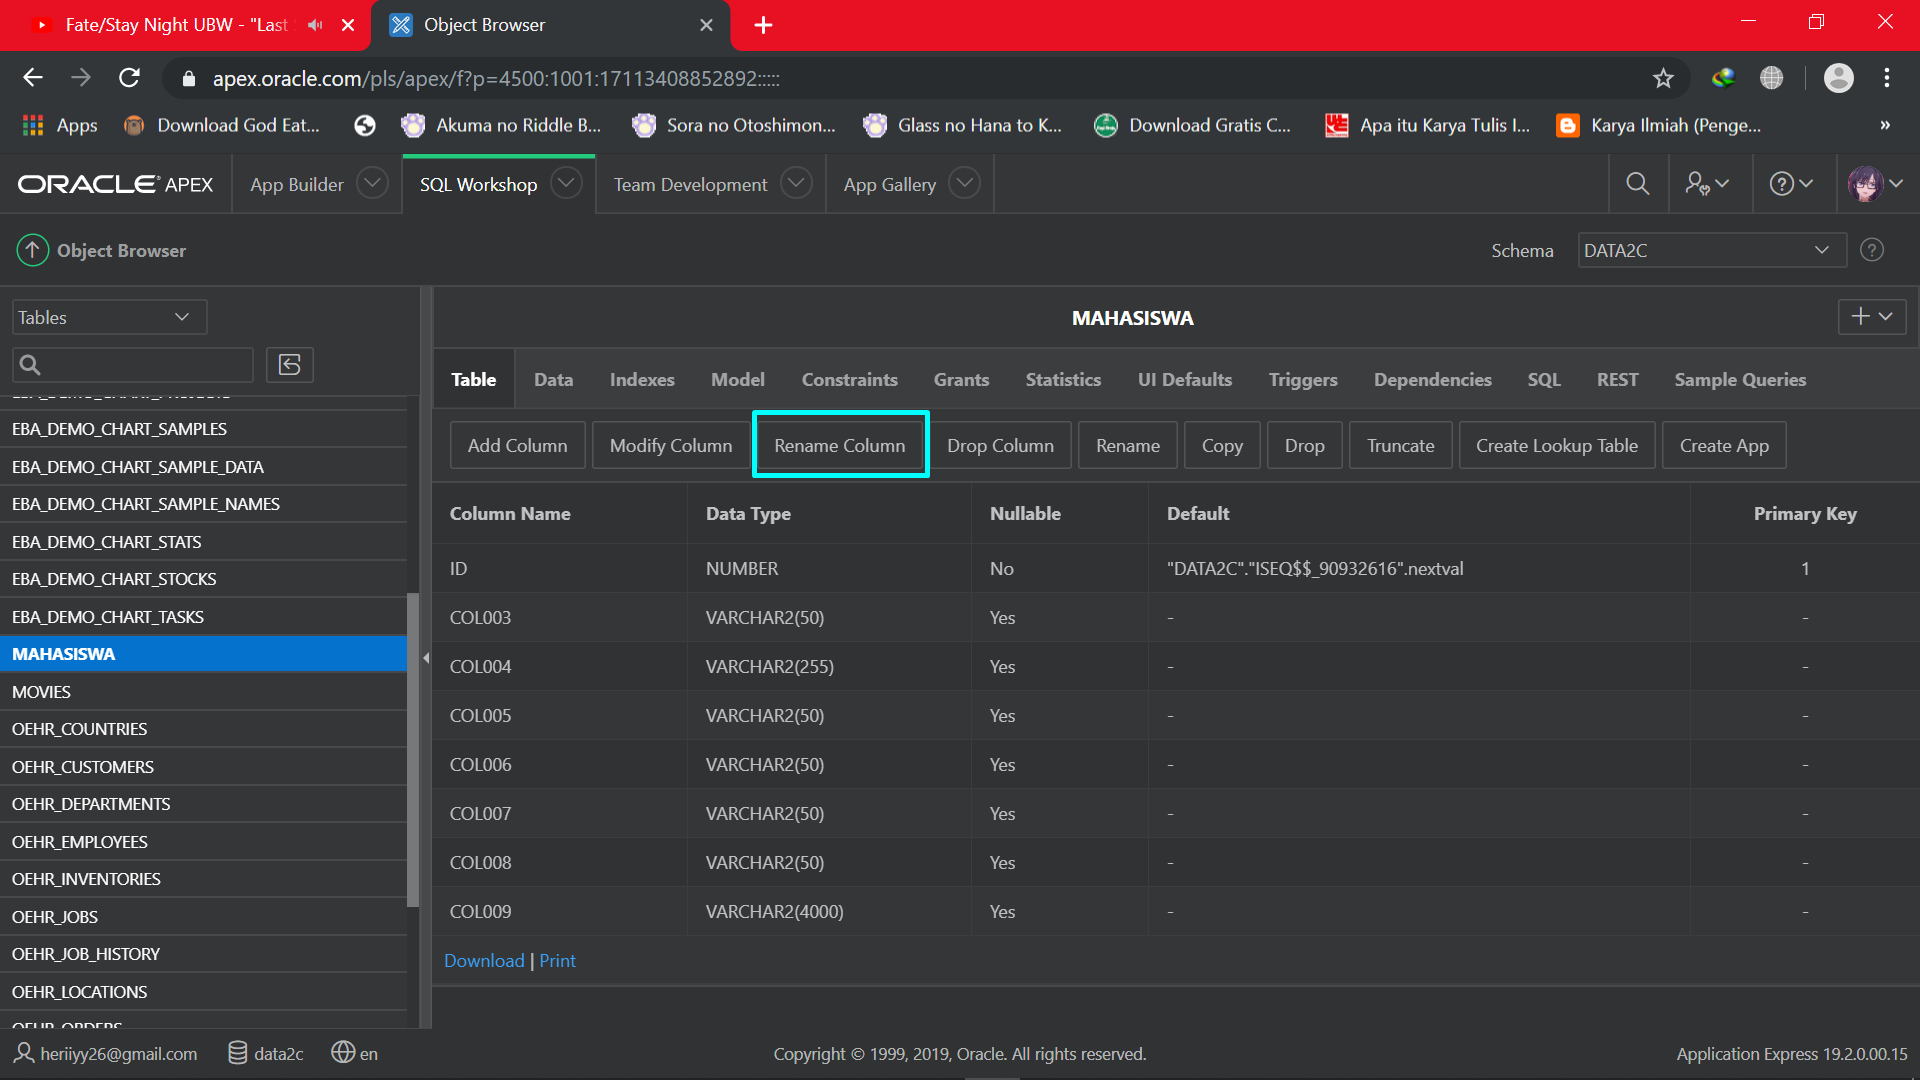
\includegraphics[width=10cm]{figures/14.png}
	\caption{Rename Column}
\end{figure}
\item Pada kotak "Curent Column Name" pilih kolom yang ingin diganti namanya, lalu di bawahnya adalah kotak "New Column Name" ketikkan nama kolom baru untuk kolom yang ingin diganti namanya.
\begin{figure}[htbp]
	\centering
	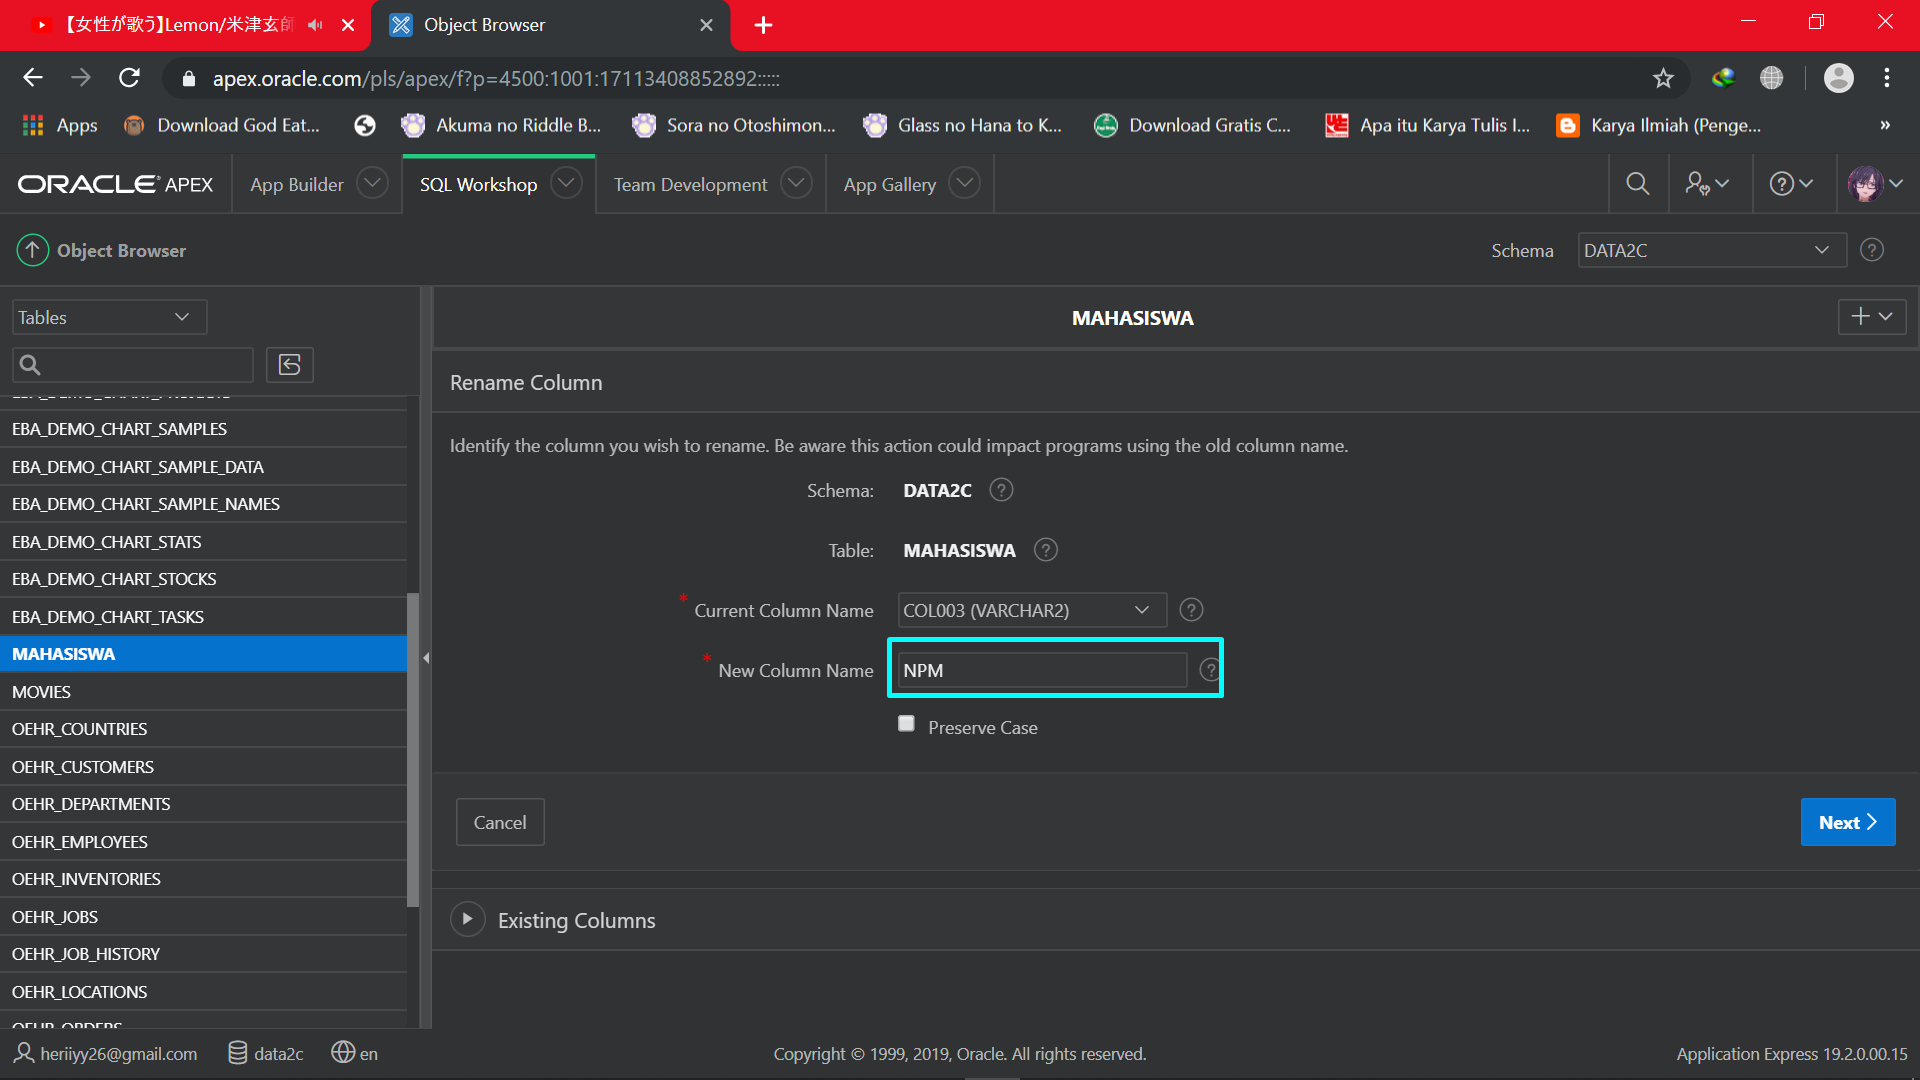
\includegraphics[width=10.5cm]{figures/15.png}
	\caption{Mengubah nama kolom}
\end{figure}
\item Selanjutnya akan dialihkan ke halaman Confirm, klik "Finish" untuk selesai mengganti nama. Lakukan hal yang sama pada setiap kolom.
\begin{figure}[htbp]
	\centering
	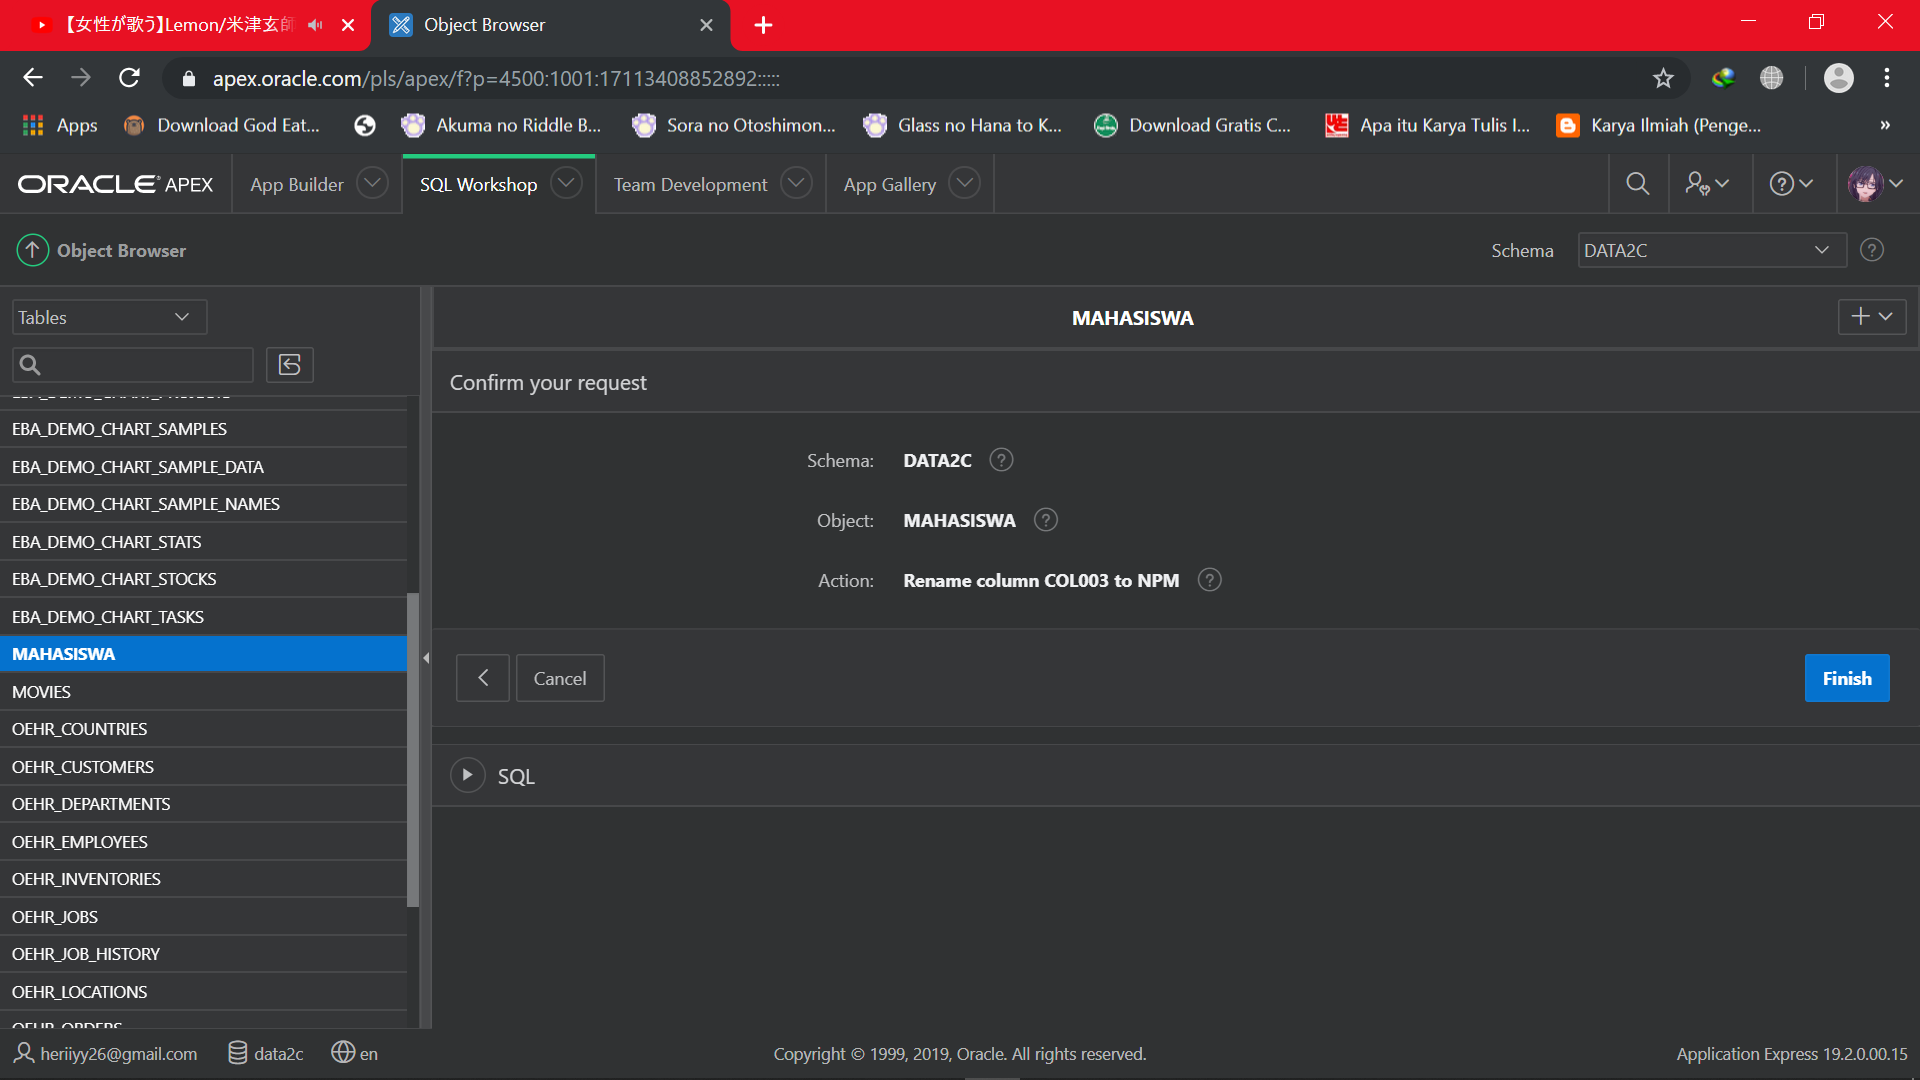
\includegraphics[width=10.5cm]{figures/16.png}
	\caption{Konfirmasi nama kolom baru}
\end{figure}
\item Pada gambar di bawah nama kolom telah diubah semua.
\begin{figure}[htbp]
	\centering
	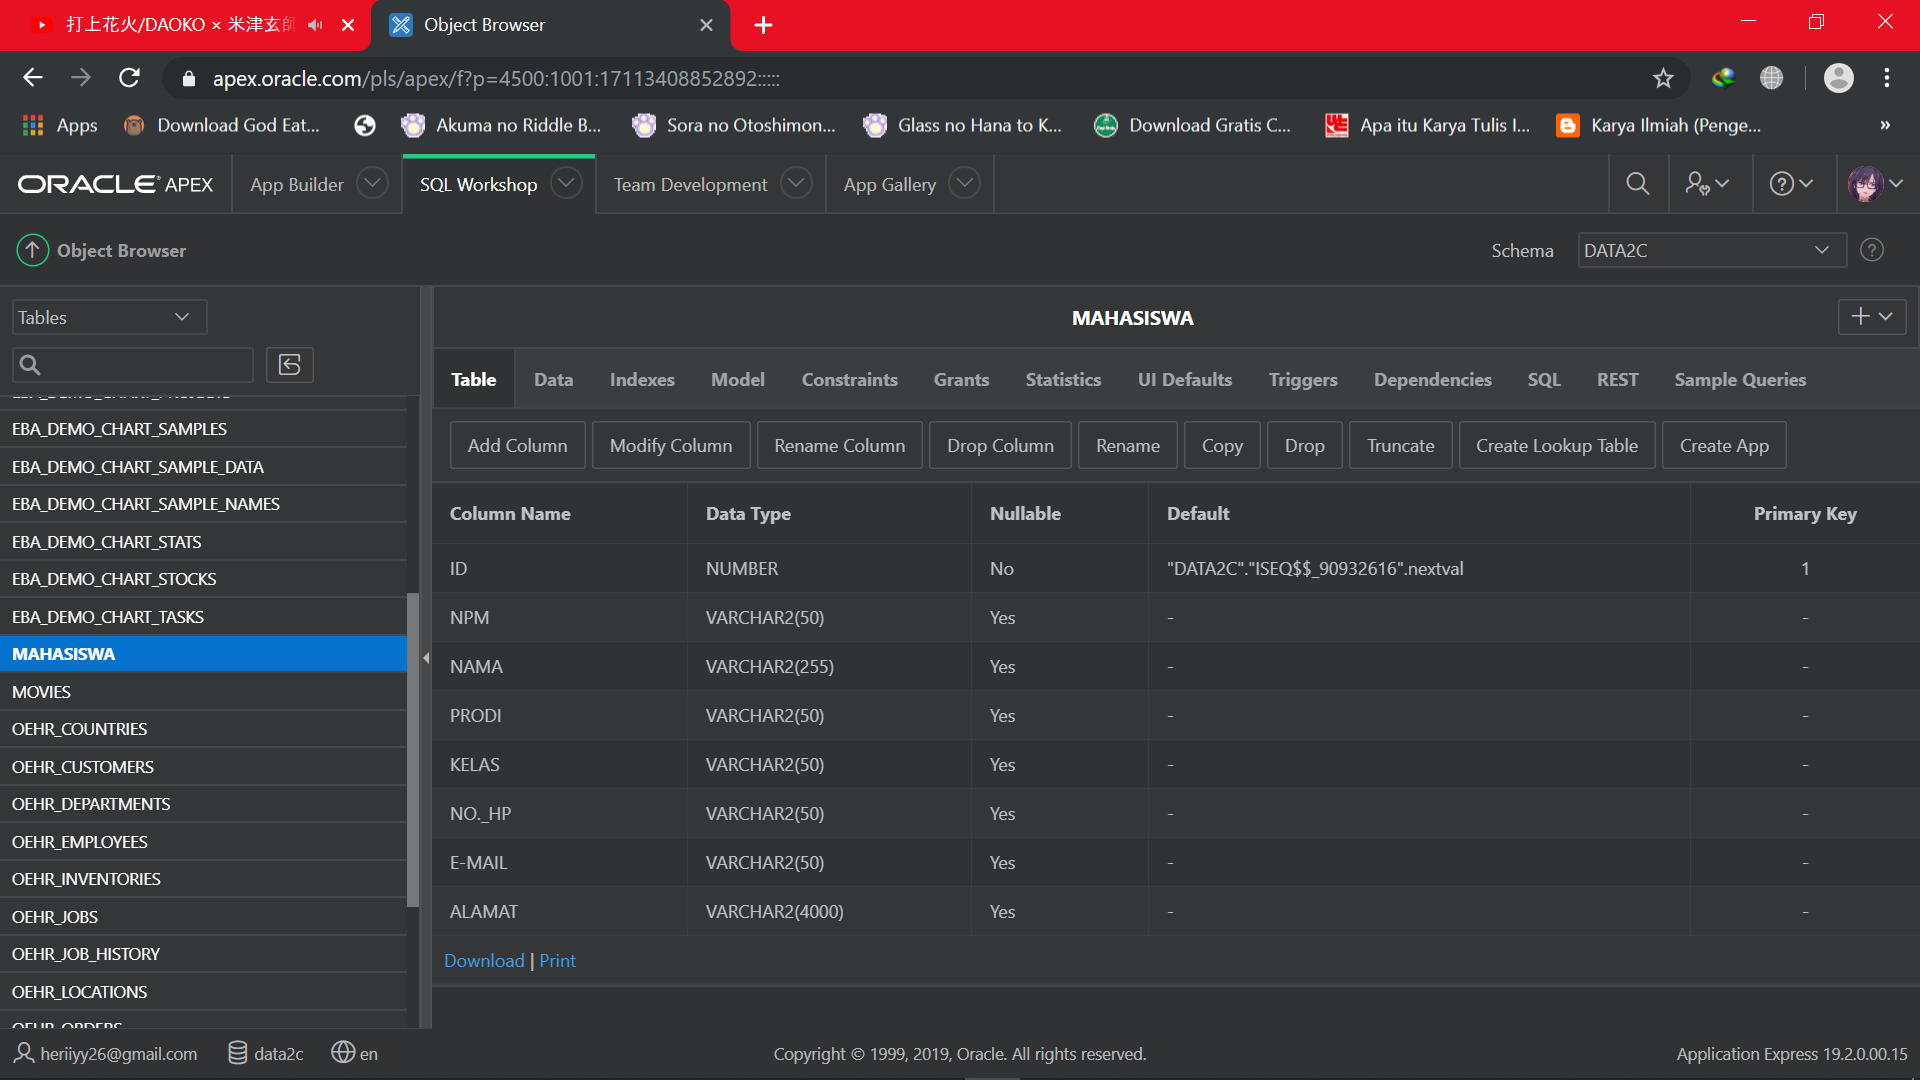
\includegraphics[width=10.5cm]{figures/18.png}
	\caption{Nama Kolom Baru}
\end{figure}\\
\\
\item Selanjutnya mengubah data pada row ke-1 pada tabel mahasiswa dengan data mahasiswa. Caranya adalah klik tombol "Edit" disamping data.
\begin{figure}[htbp]
	\centering
	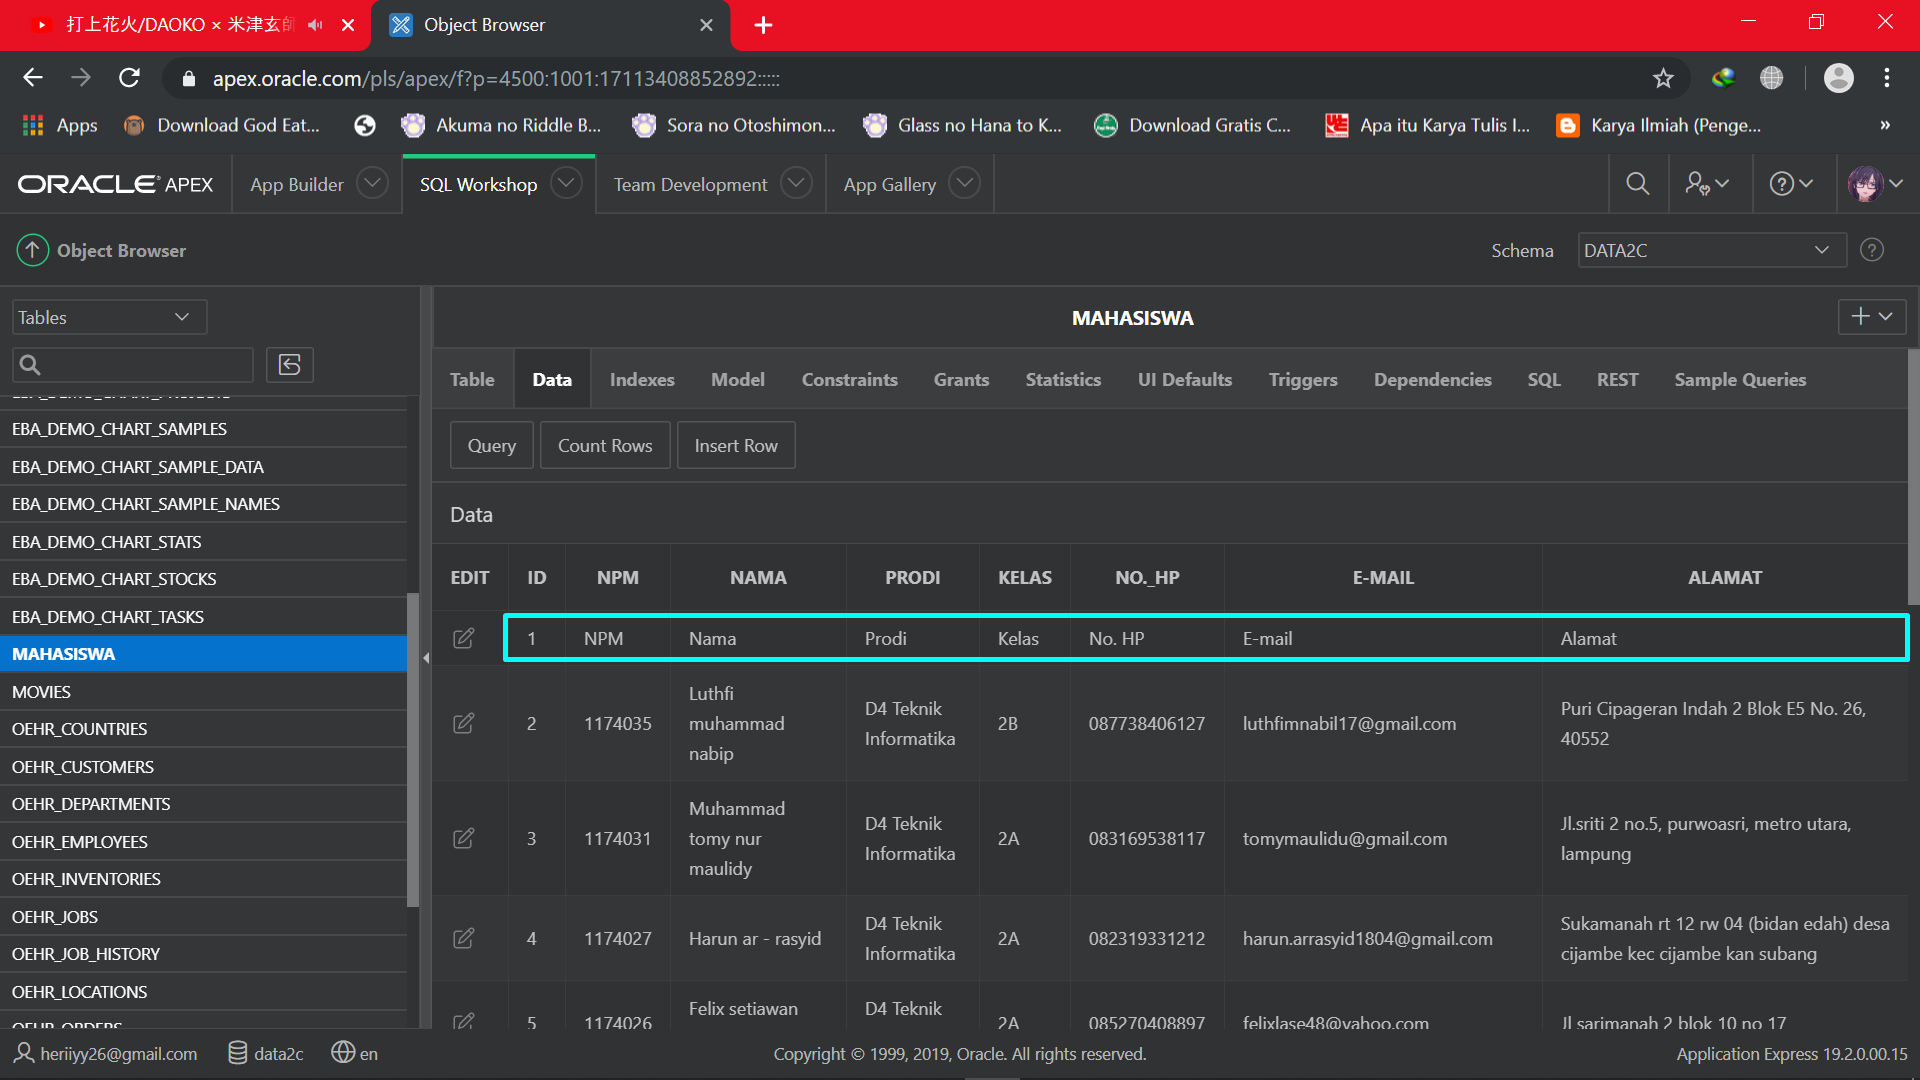
\includegraphics[width=10.5cm]{figures/19.png}
	\caption{Mengubah data row 1}
\end{figure}
\item Selanjutnya akan dialihkan ke halaman Edit Row, silahkan isi datanya sesuai dengan perintah yang ada, jika sudah klik "Apply Chages" di sudut kanan atas.
\begin{figure}[htbp]
	\centering
	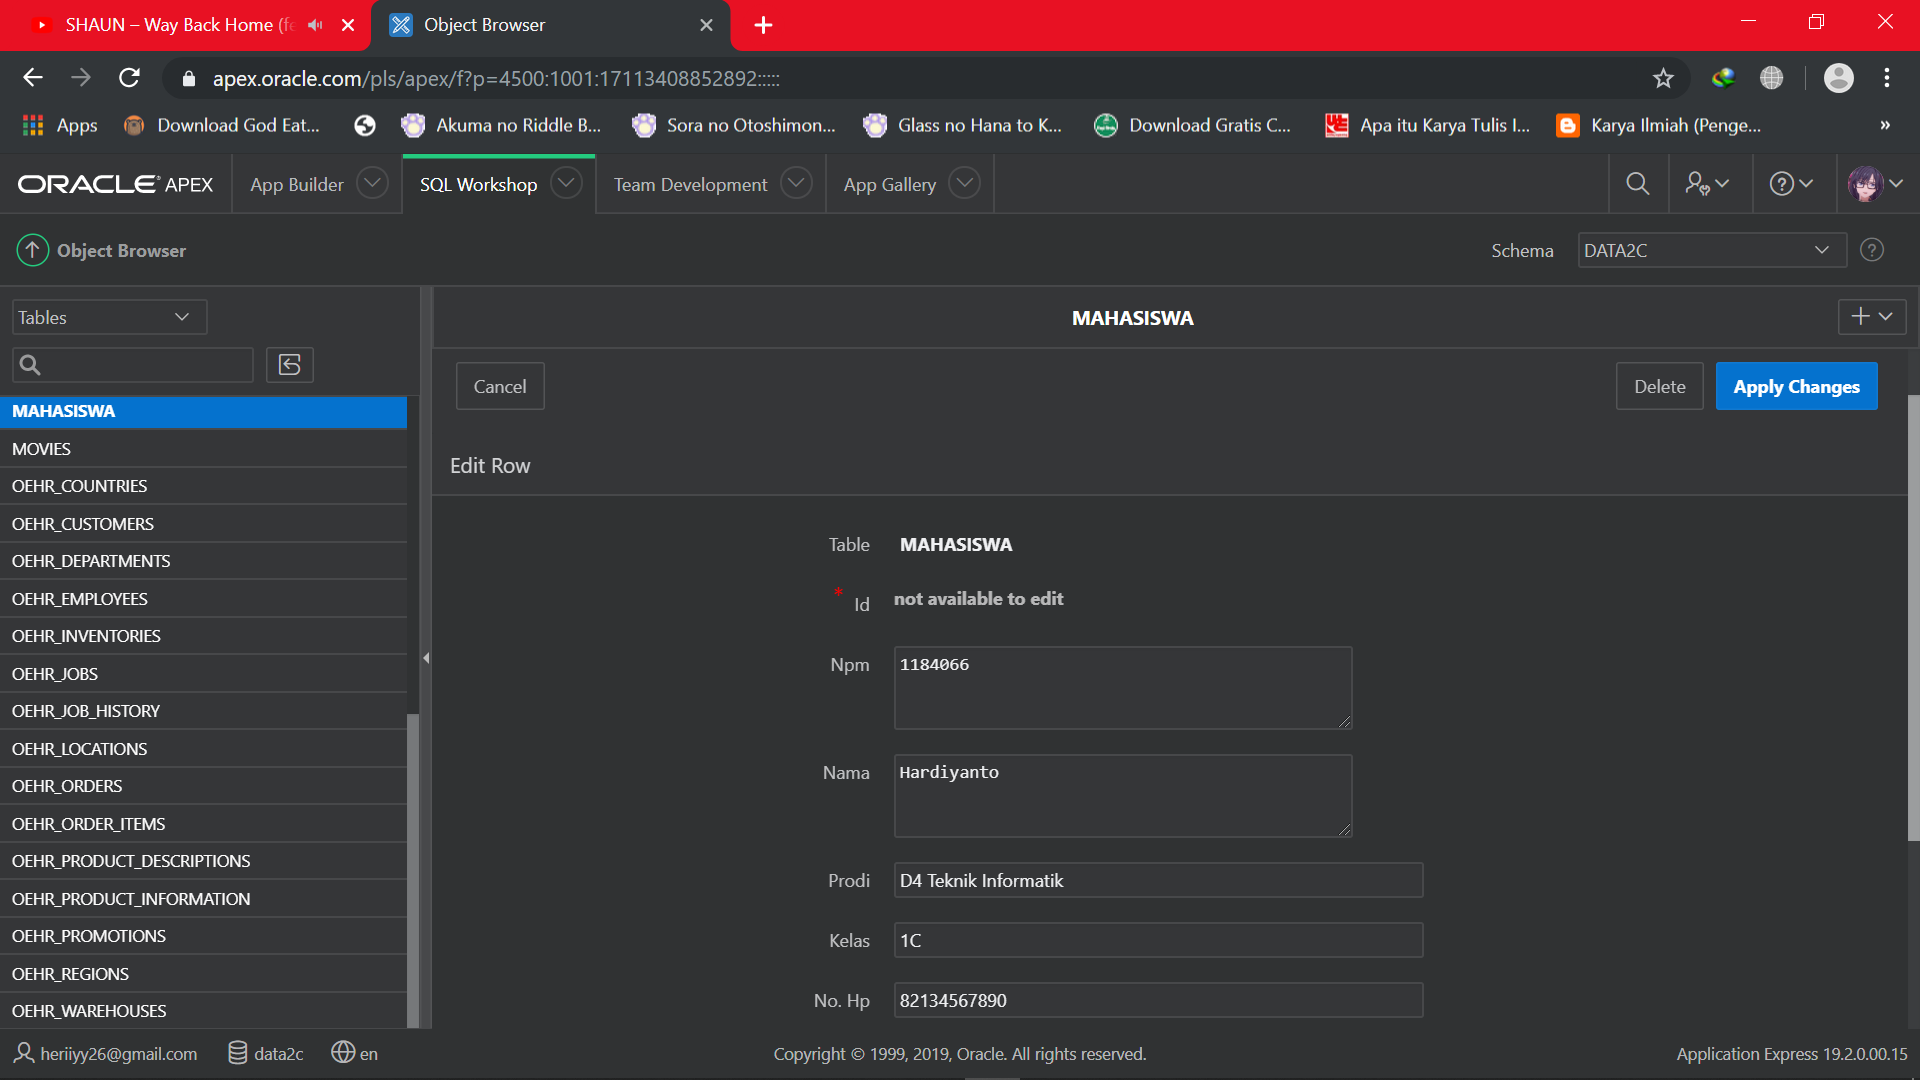
\includegraphics[width=10cm]{figures/20.png}
	\caption{Mengisi form edit row}
\end{figure}\\
\item Sekarang tabel mahasiswa sudah benar dan rapi.
\begin{figure}[htbp]
	\centering
	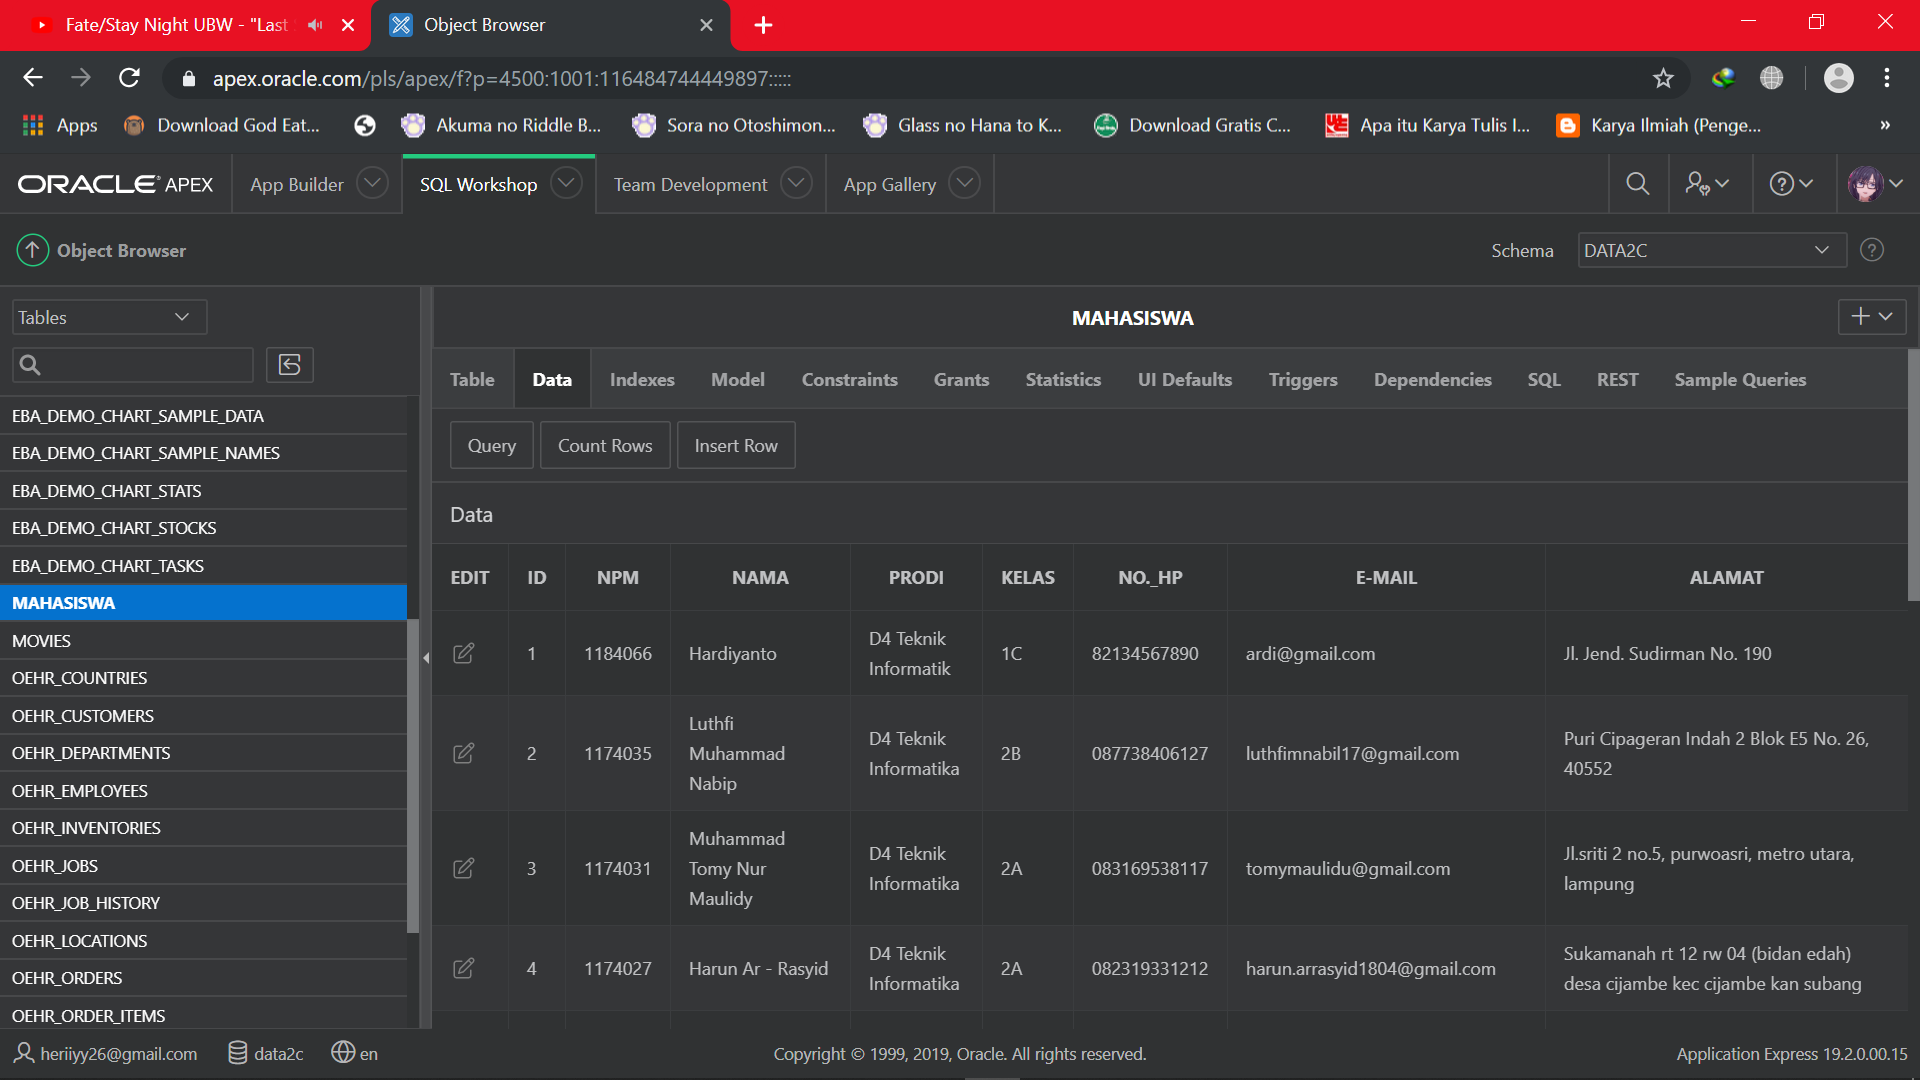
\includegraphics[width=10.5cm]{figures/21.png}
	\caption{Tabel Mahasiswa}
\end{figure}
\item Sekarang kita akan membuat aplikasinya, caranya adalah klik tab tabel, pada tab table klik "Create App".
\begin{figure}[htbp]
	\centering
	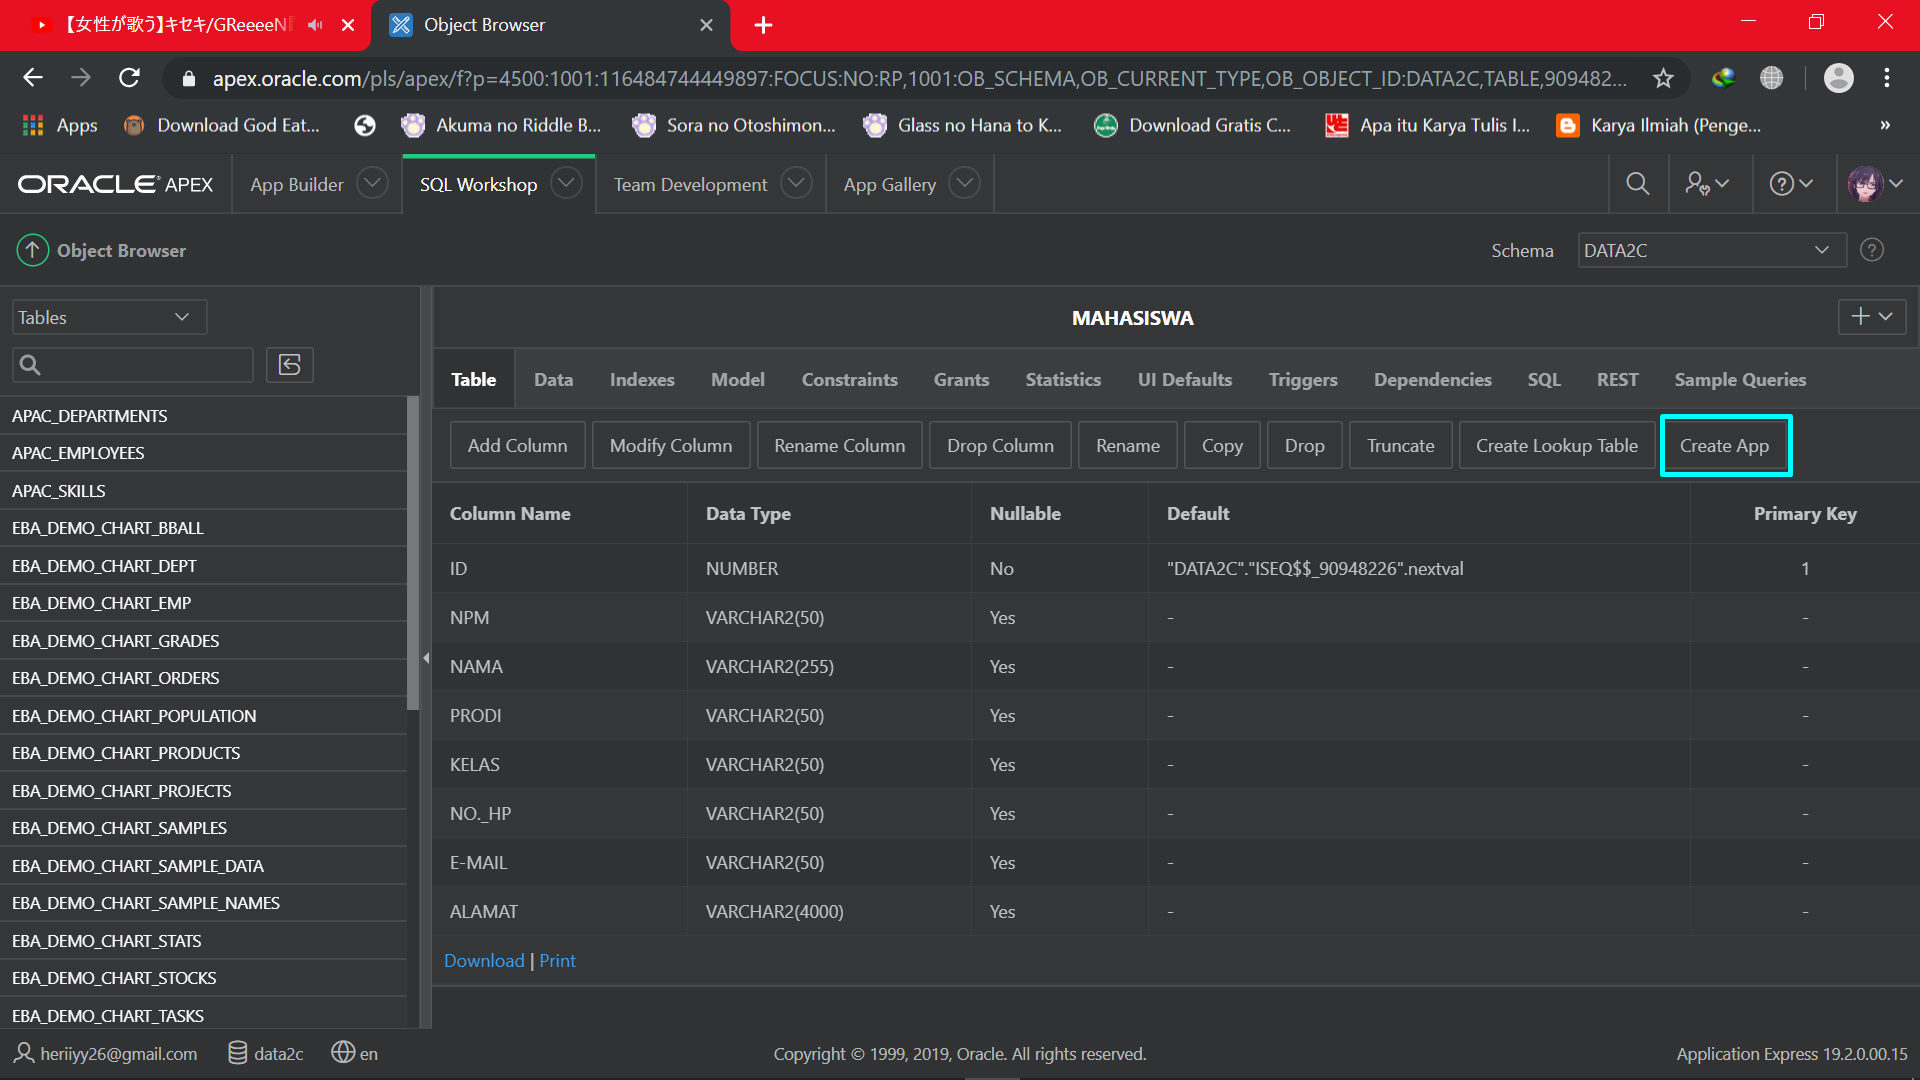
\includegraphics[width=10.5cm]{figures/22.png}
	\caption{Membuat Aplikasi}
\end{figure}\\
\\
\\
\item Selanjutnya akan dialihkan pada halaman Create Application, klik "Create App".
\begin{figure}[htbp]
	\centering
	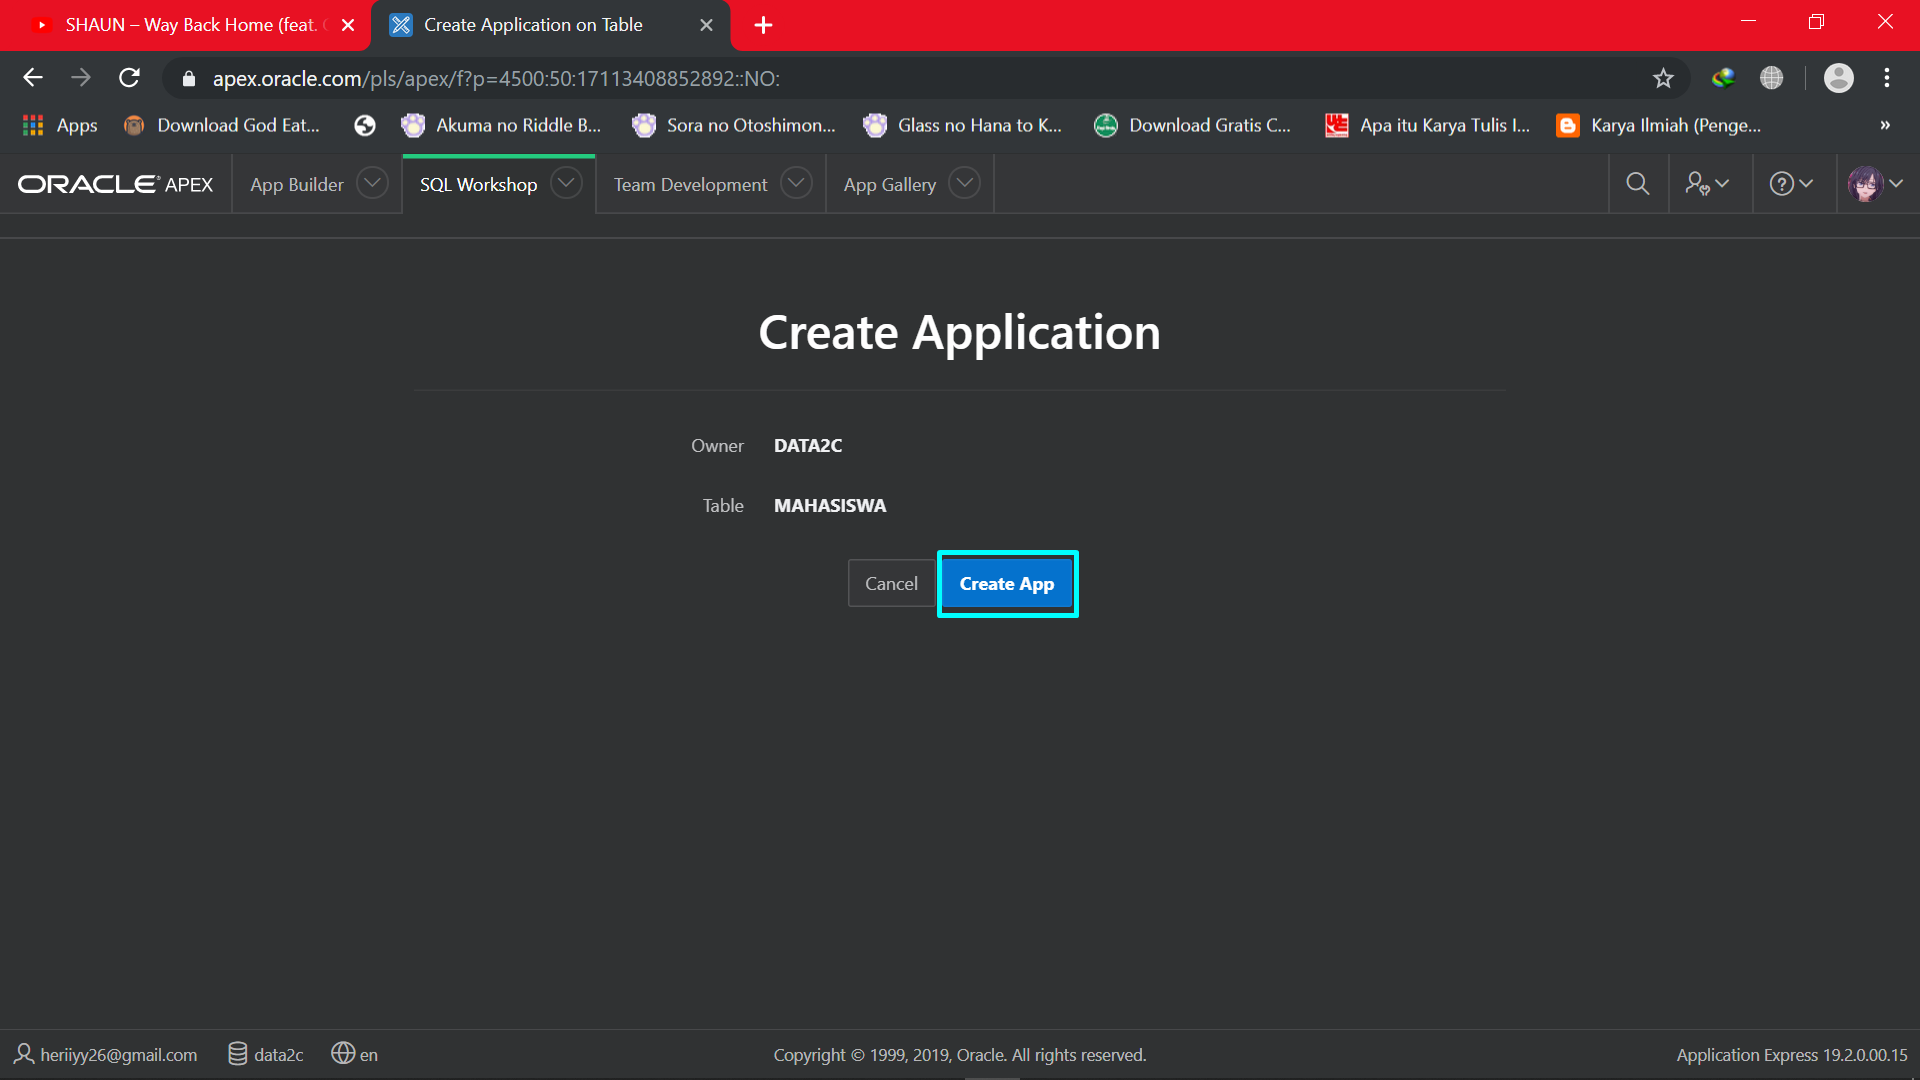
\includegraphics[width=10.5cm]{figures/23.png}
	\caption{Membuat Aplikasi}
\end{figure}
\item Selanjutnya akan dialihkan pada halaman Create an Application, isinya nama aplikasi dengan nama "Mahasiswa App" pada kotak "Name".
\begin{figure}[htbp]
	\centering
	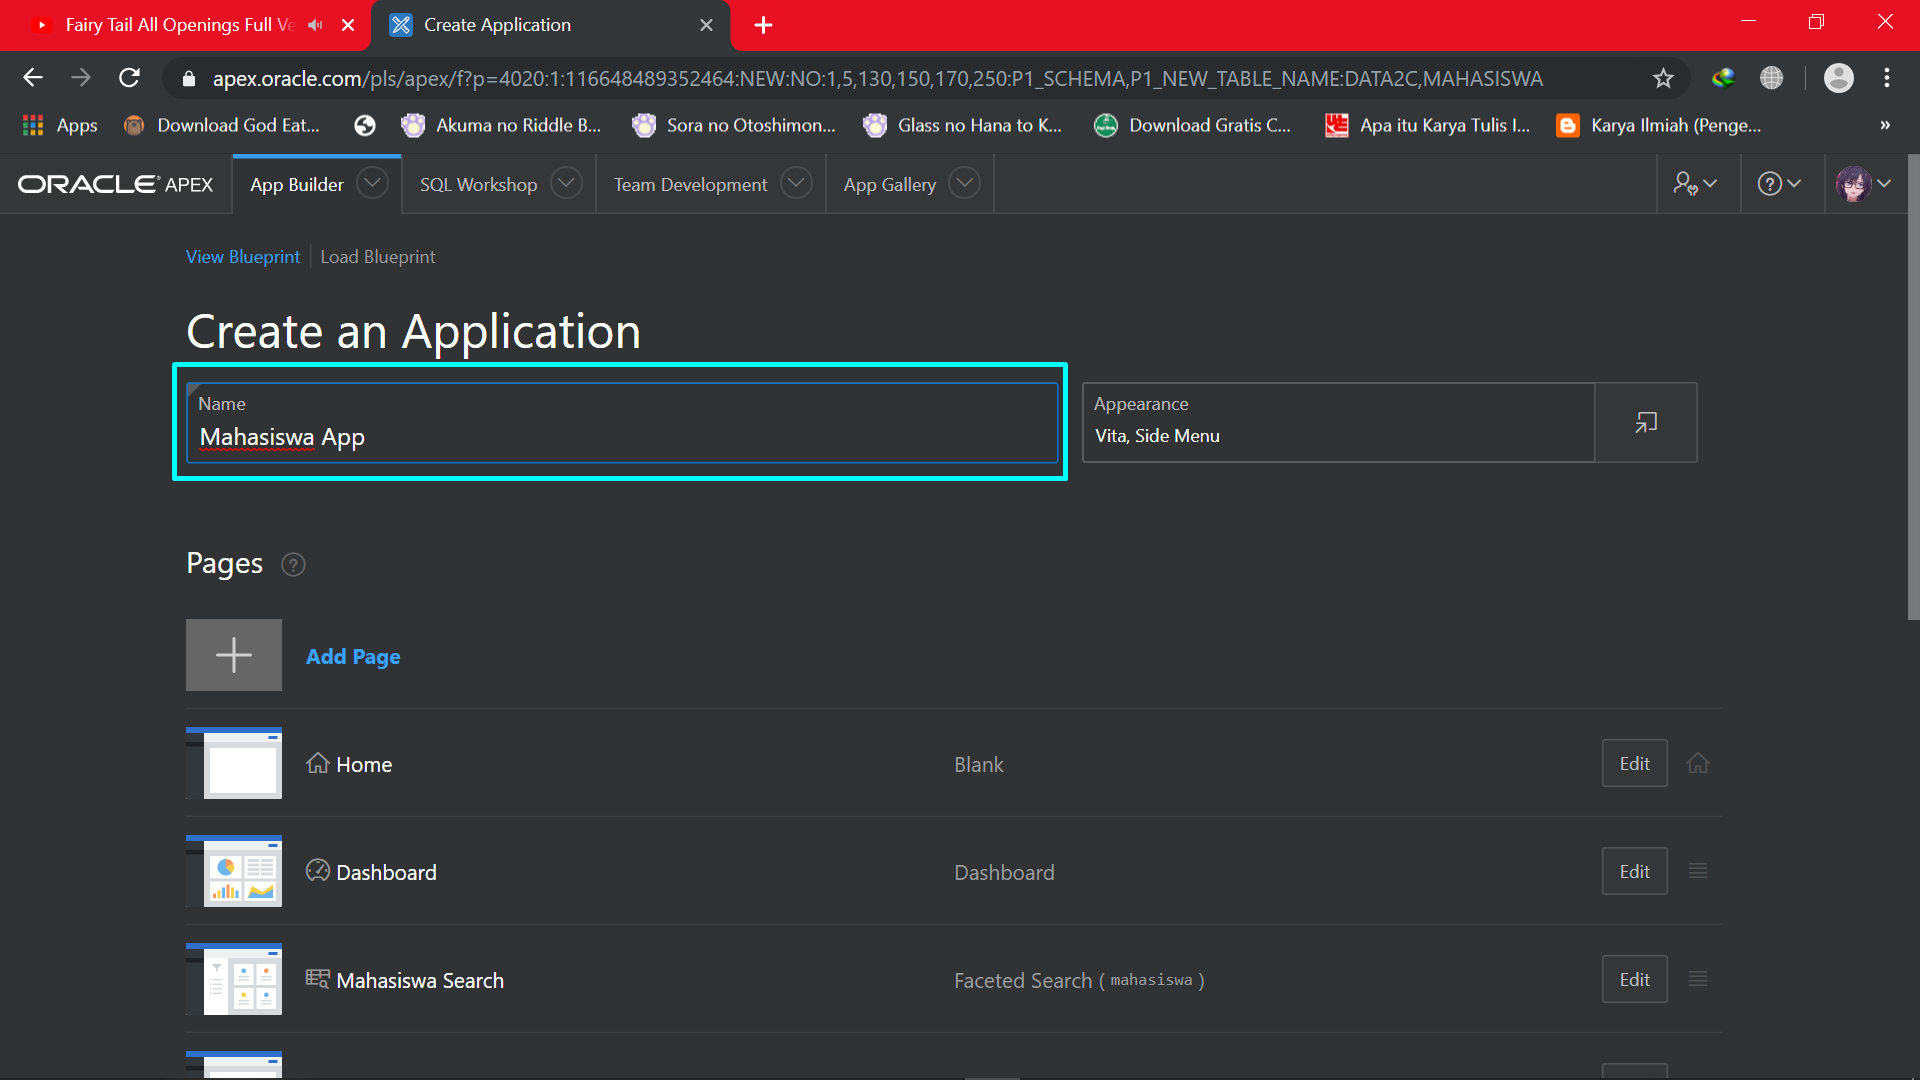
\includegraphics[width=10.5cm]{figures/24.png}
	\caption{Memberi nama Aplikasi}
\end{figure}\\
\\
\item Tetap pada halaman yang sama, scroll halaman ke bawah, pada features klik "Check All", agar kita dapat menggunakan semua fitur dari aplikasi, jika sudah klik "Create Application", tunggu proses sampai selesai.
\begin{figure}[htbp]
	\centering
	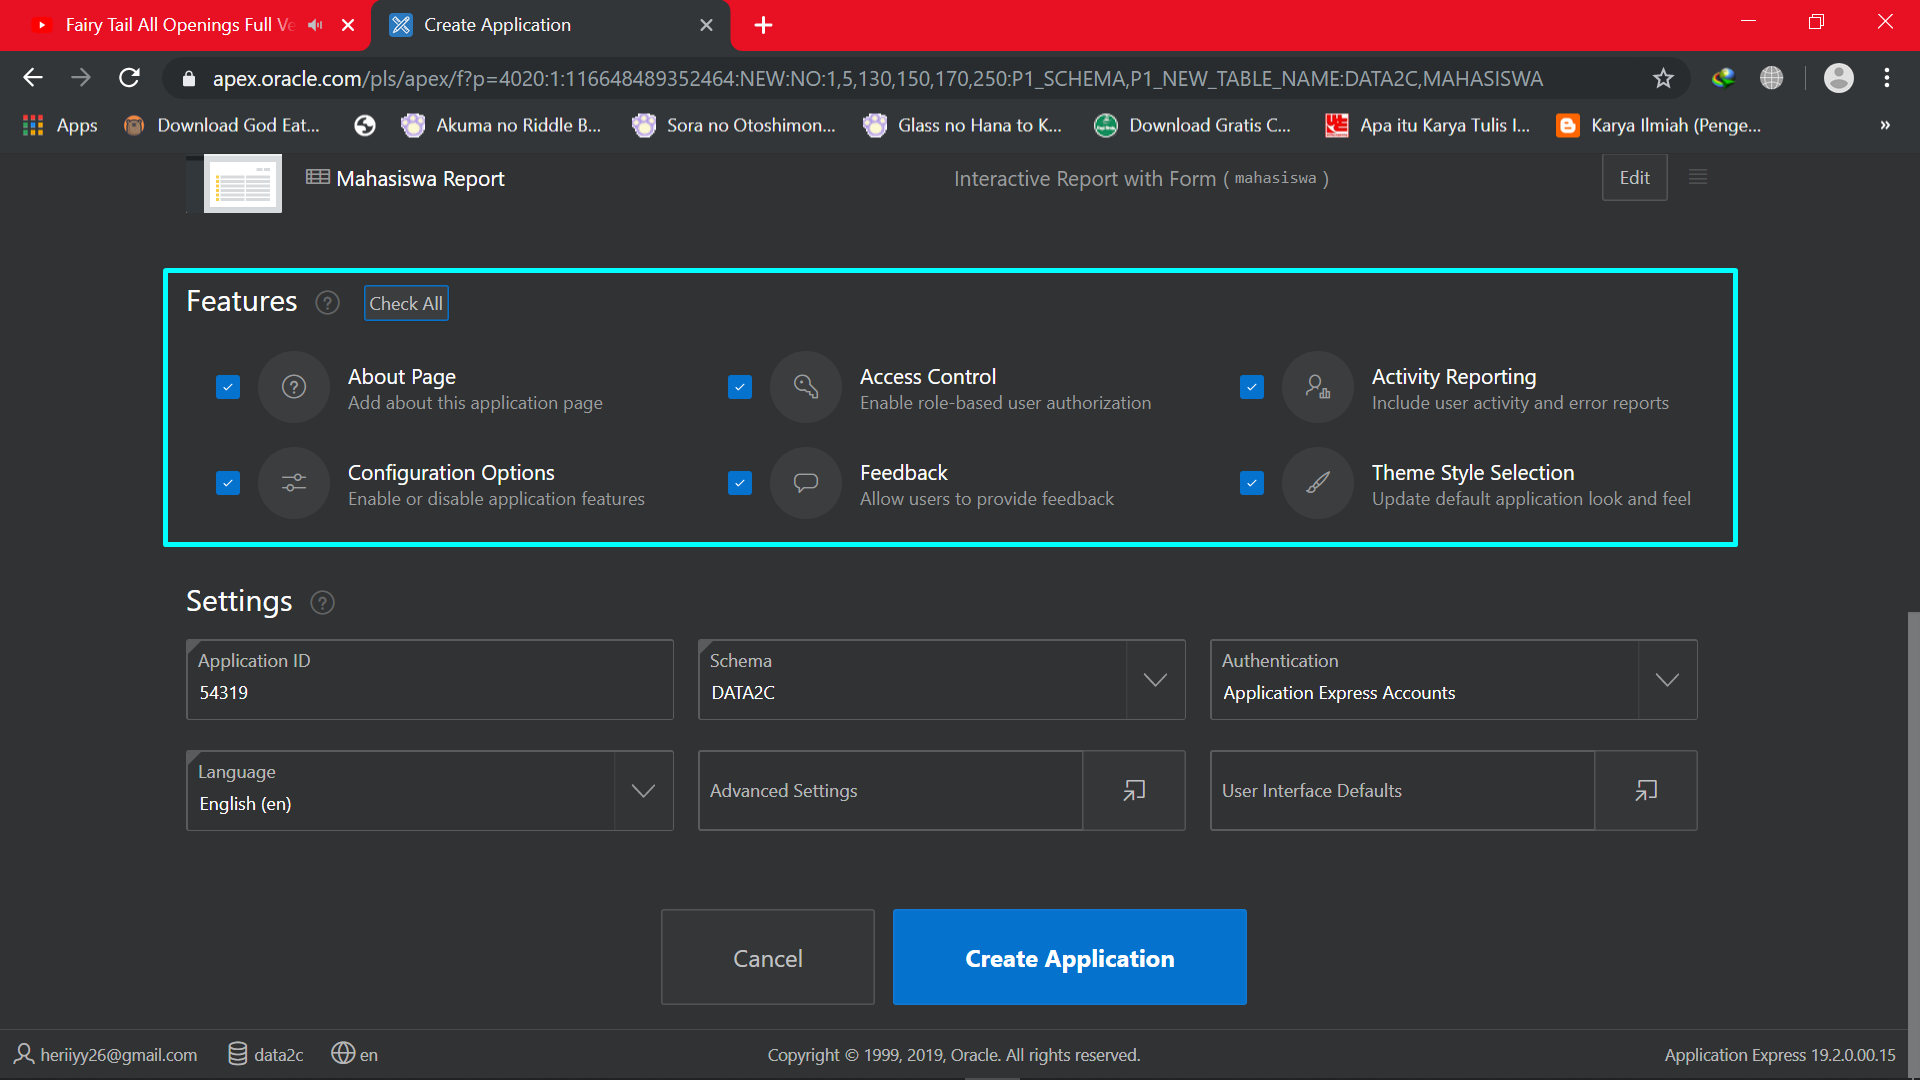
\includegraphics[width=10.5cm]{figures/25.png}
	\caption{Membuat Aplikasi}
\end{figure}
\item Aplikasi sudah selesai dibuat dan siap dijalankan. Klik "Run Application" untuk menjalankan aplikasi.
\begin{figure}[htbp]
	\centering
	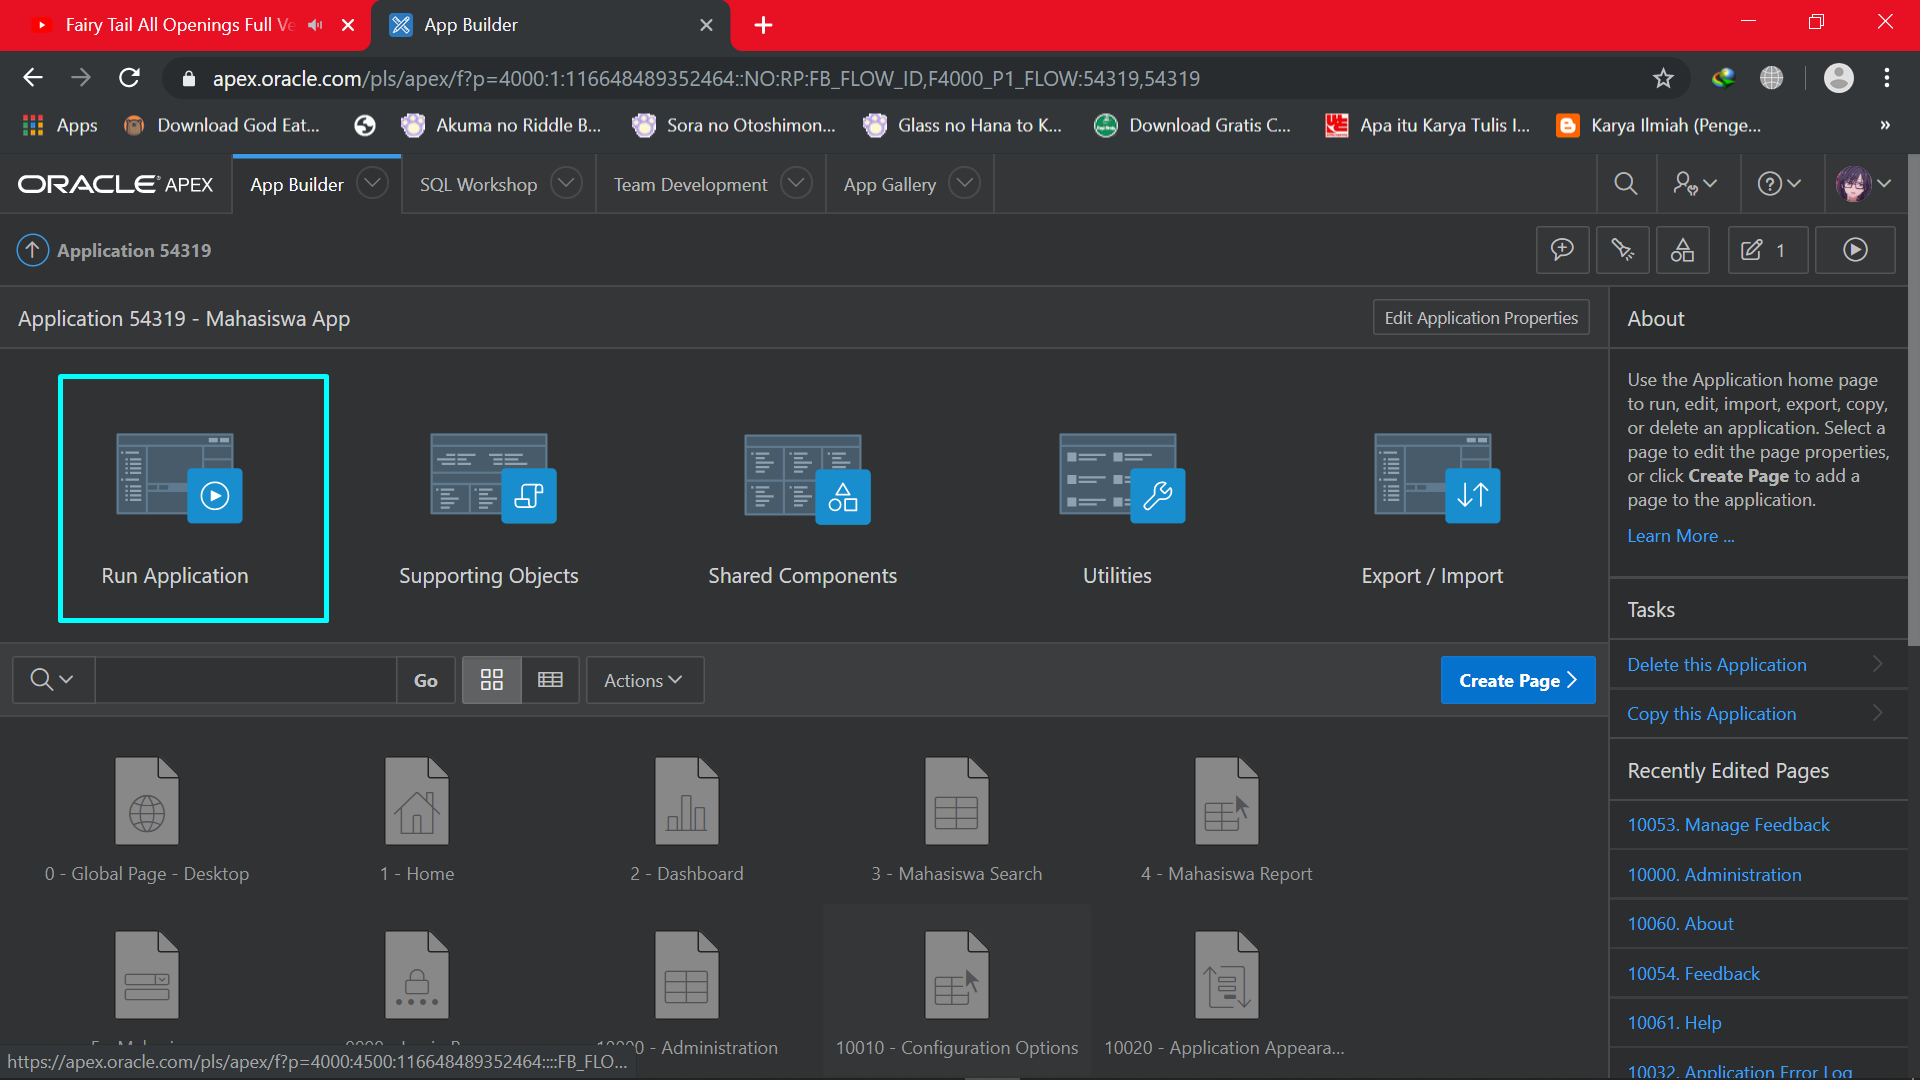
\includegraphics[width=10.5cm]{figures/26.png}
	\caption{Run Application}
\end{figure}
\item Aplikasi sudah jalan, silahkan login sesuai dengan akun apex.oracle anda.
\begin{figure}[htbp]
	\centering
	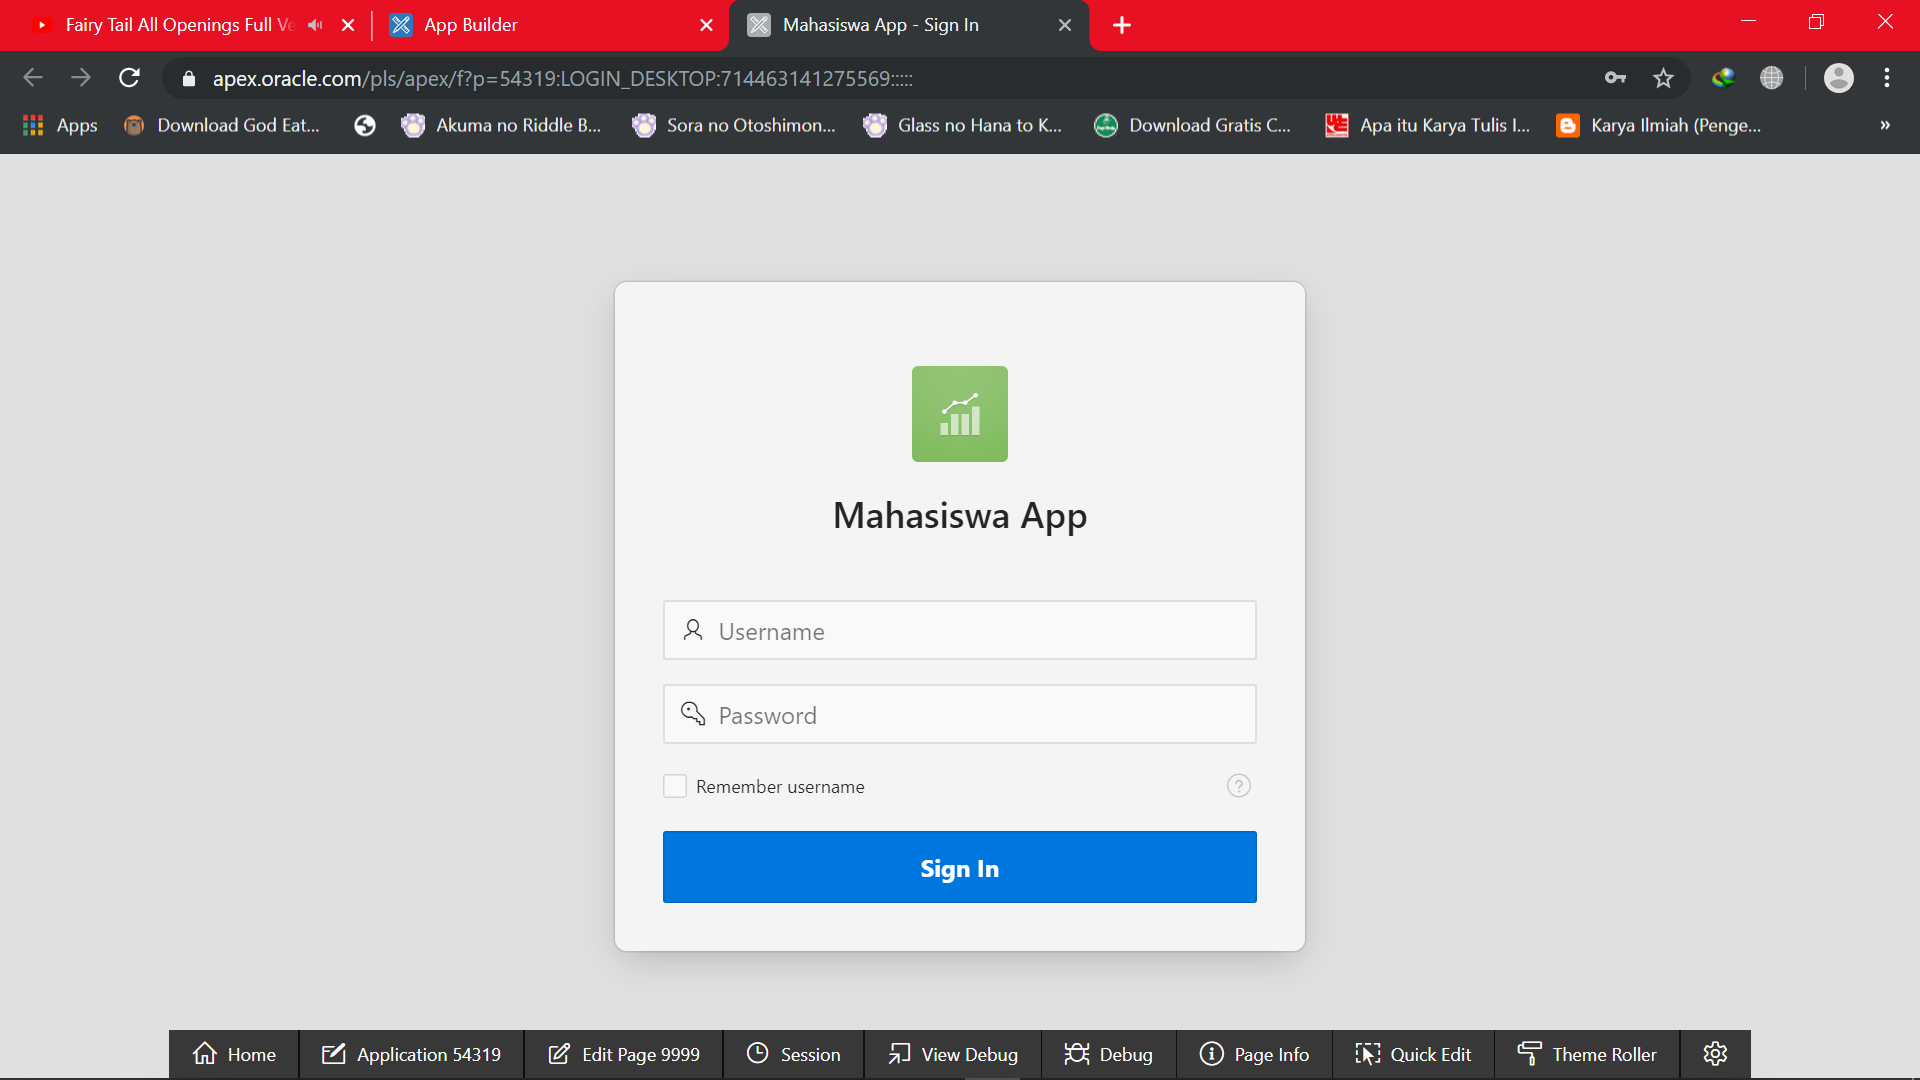
\includegraphics[width=10.5cm]{figures/27.png}
	\caption{Login ke Aplikasi}
\end{figure}
\item Tampilan halaman Dashboard Aplikasi.
\begin{figure}[htbp]
	\centering
	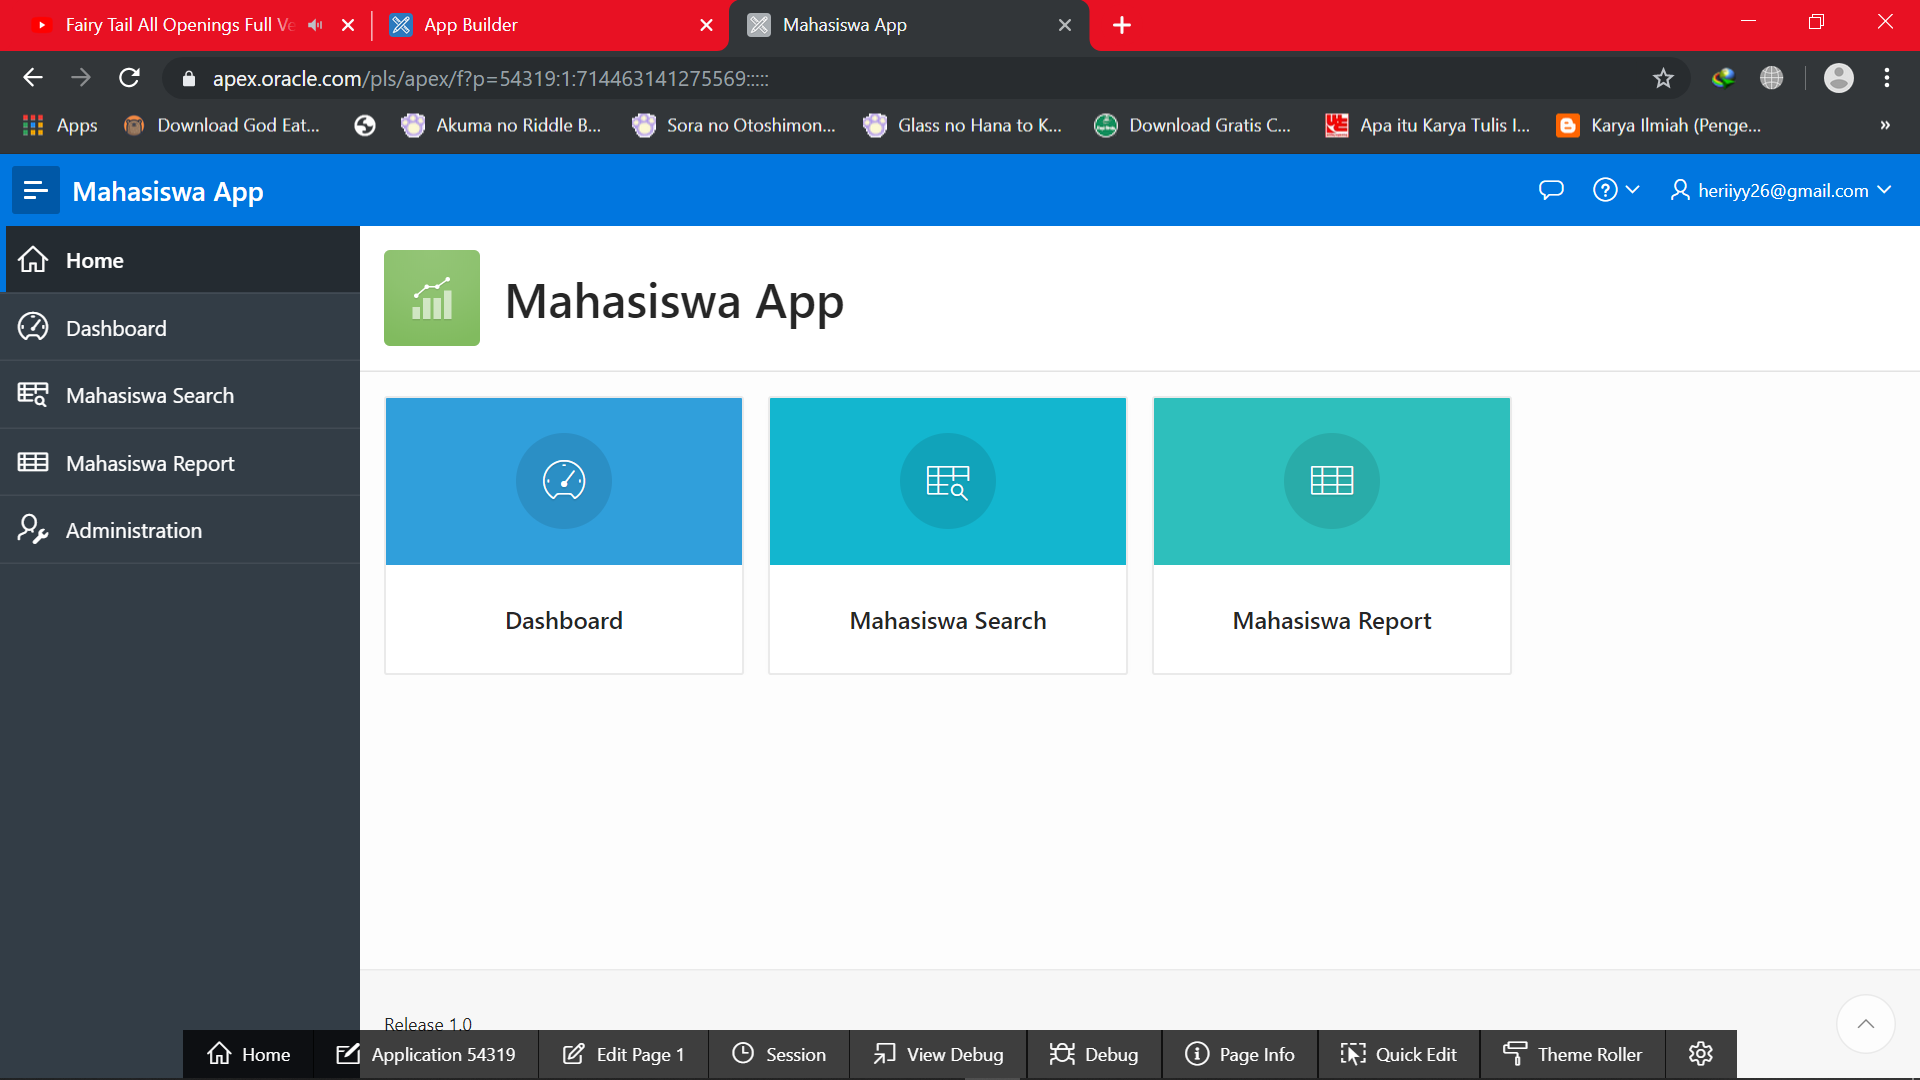
\includegraphics[width=10.5cm]{figures/28.png}
	\caption{Interface Dashboard}
\end{figure}
\\
\\
\\
\item Tampilan halaman Mahasiswa Search. Di halaman ini kita dapat mencari data mahasiswa berdasarkan nama atau lainnya dengan cepat.
\begin{figure}[htbp]
	\centering
	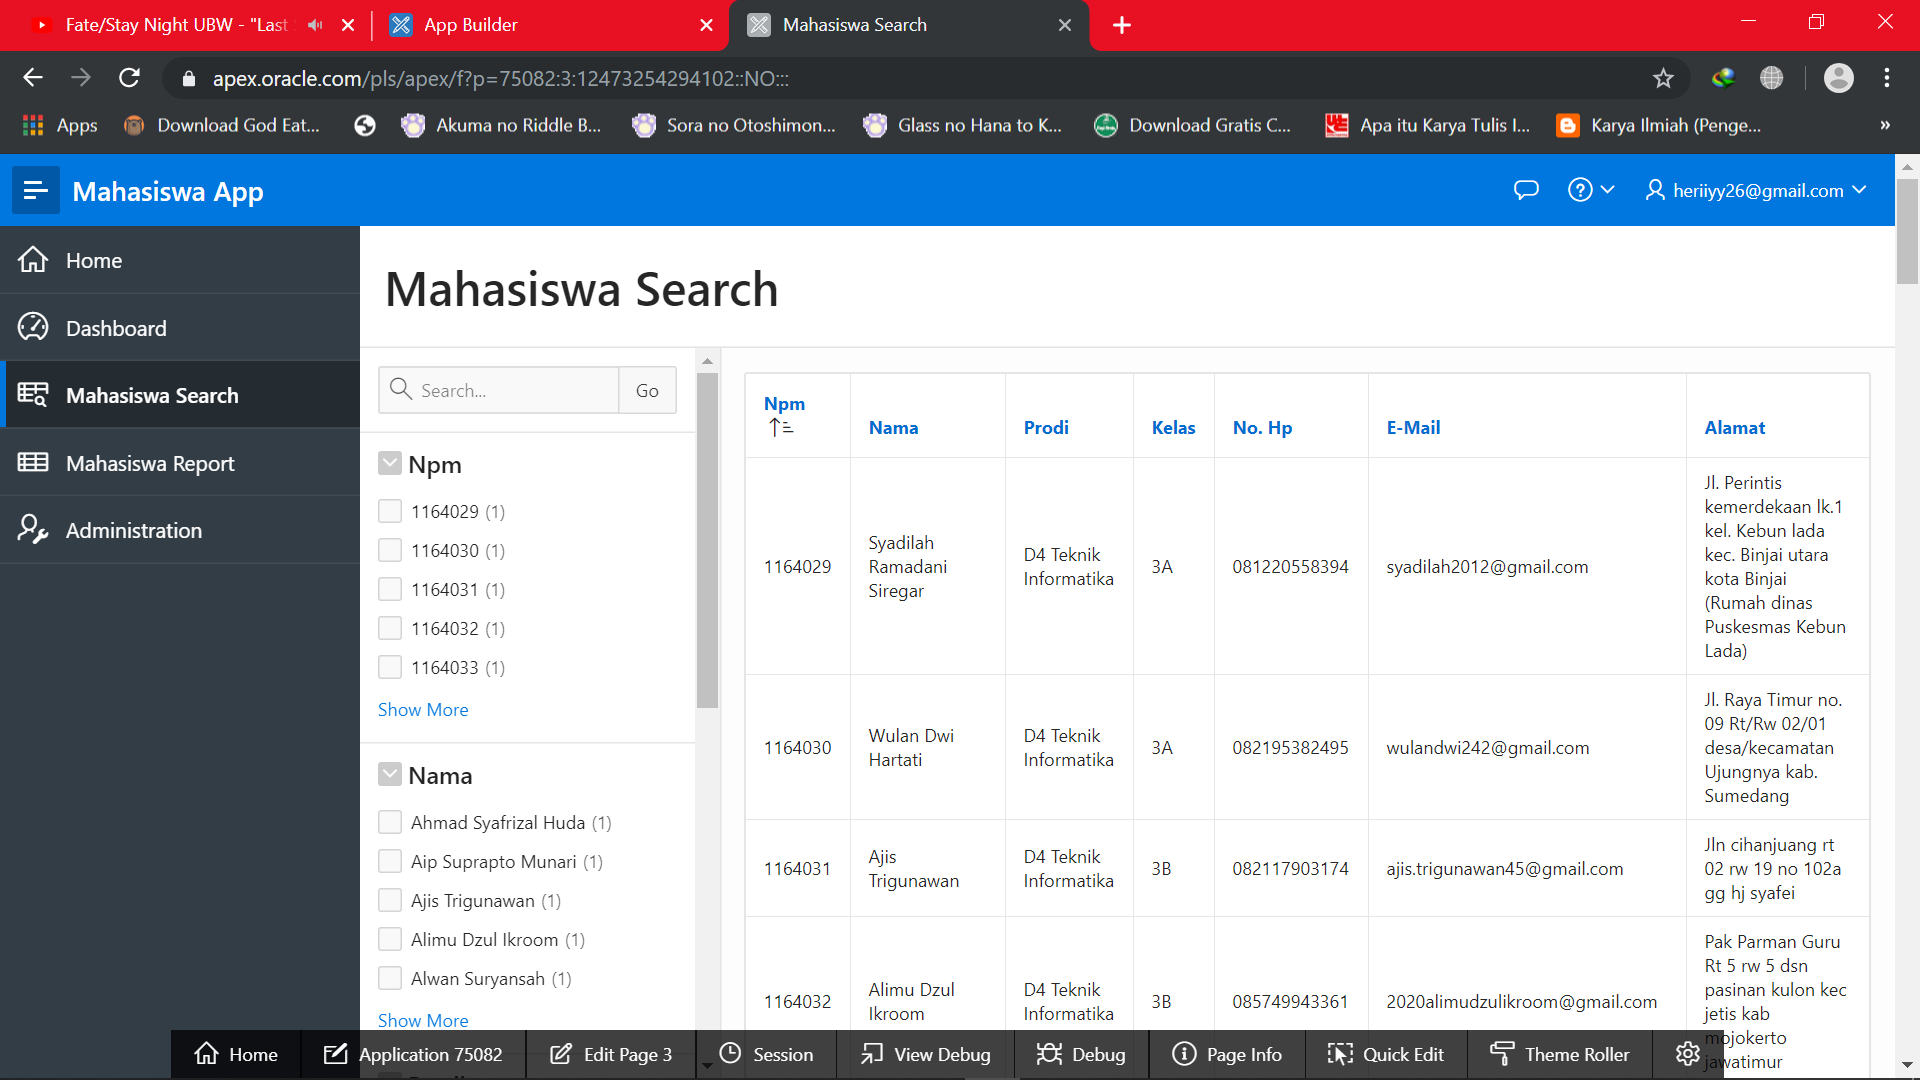
\includegraphics[width=10.5cm]{figures/29.png}
	\caption{Interface Mahasiswa Search}
\end{figure}
\item Tampilan halaman Mahasiswa Report. Di halaman ini kita dapat mengubah data mahasiswa menambah atau menghapus data mahasiswa di halaman ini.
\begin{figure}[htbp]
	\centering
	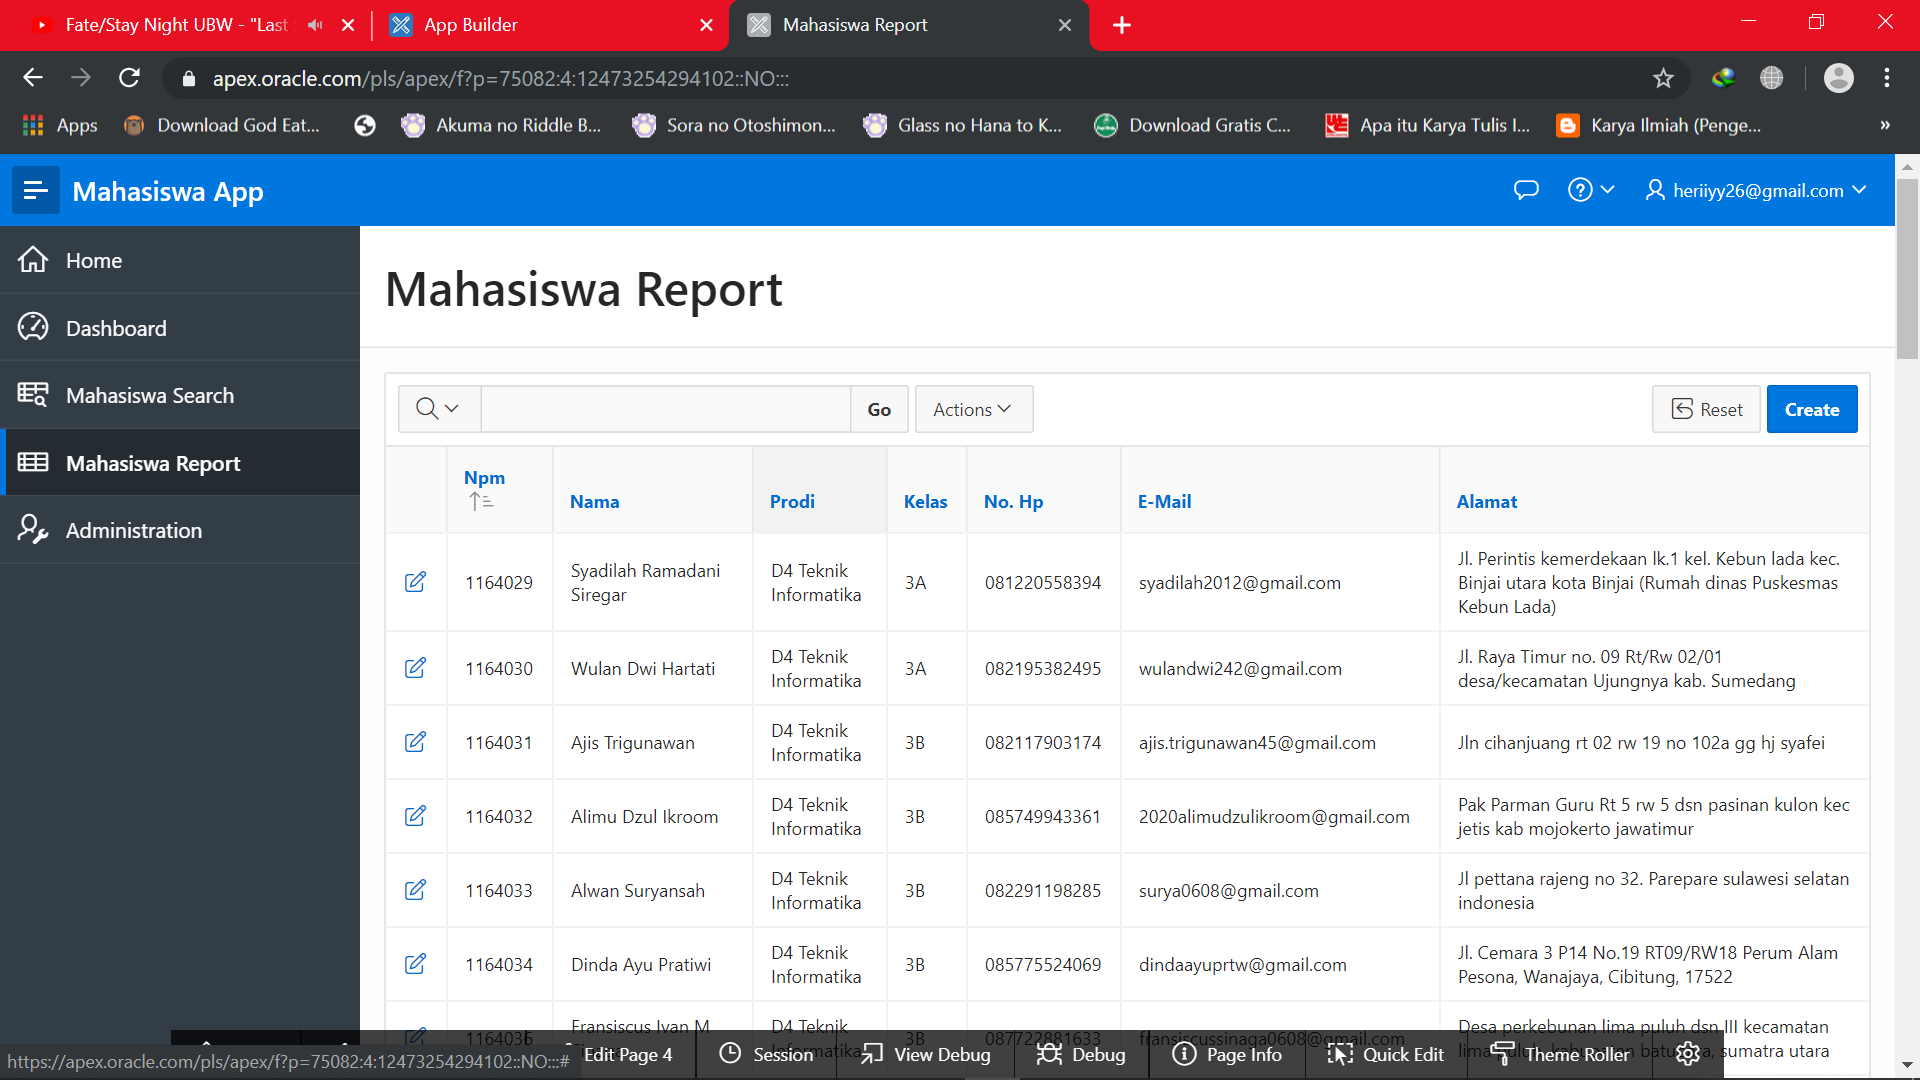
\includegraphics[width=10.5cm]{figures/30.png}
	\caption{Interface Mahasiswa Report}
\end{figure}\\
\item Tampilan halaman Administration. Di halaman ini kita dapat mengkostumisasi aplikasi kita dari warna, tampilan, dan lain-lain
\begin{figure}[htbp]
	\centering
	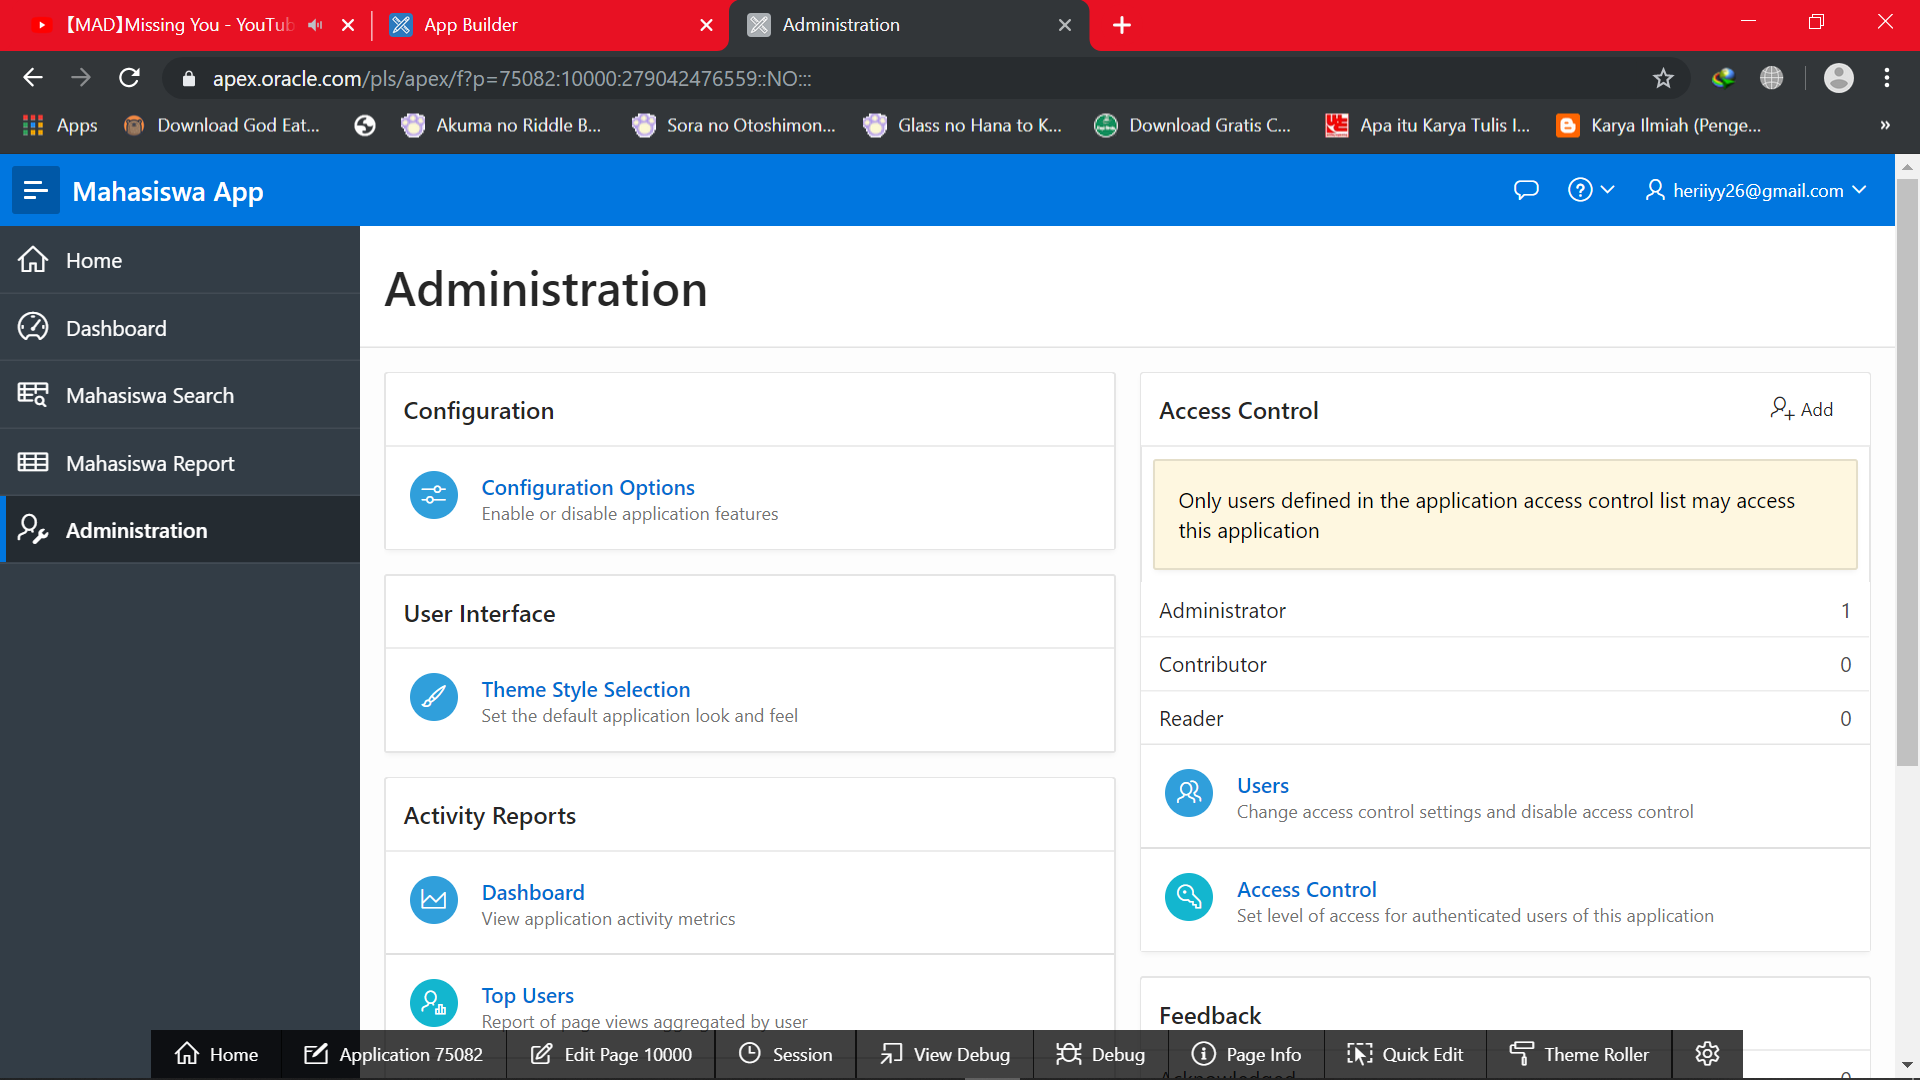
\includegraphics[width=12cm]{figures/31.png}
	\caption{Interface Administation}
\end{figure}
\end{itemize}
\section{Note}
\begin{itemize}
\item Workspace = data2c
\item Username = heriiyy26@gmail.com
\item Password = makioshi194
\end{itemize}

\end{document}